\chapter{Úvod}
TODO

%=========WATERMARKING========
\chapter{Watermarking}
Watermarking je proces skrývania digitálnej informácie do nosného signálu.

Na jednej strane je watermarking blízko spätý so steganografiou, ale na druhej strane je založený na iných základných filozofiách, potrebách a aplikáciách. To má za následok, že použité techniky svojimi vlastnosťami jasne oddeľujú watermarking od steganografie.

Steganografia aj watermarking popisujú techniky, ktoré sa používajú k~nepostrehnuteľnému sprostredkovaniu informácie pomocou vloženia tejto informácie do nosných dát. Steganografia je typicky spájaná s~ukrytím informácií pri point-to-point komunikácii medzi dvoma stranami. Metódy steganografie nie sú zvyčajne robustné voči modifikáciám dát alebo majú limitovanú robustnosť a ochranu vloženej informácie proti technickým modifikáciám, ktoré môžu nastať pri prenose dát alebo pri ich ukladaní. Ako príklad takejto modifikácie môže byť napríklad konverzia formátu, kompresia alebo konverzia digitálneho signálu na analógový.

Watermarking má dodatočnú odolnosť proti pokusom vymazať skryté dáta. Populárnou aplikáciou watermarkingu je dokázanie vlastníctva digitálnych dát prostredníctvom vloženia vyhlásenia o~autorských právach. Je nepochybné, že pre tento účel by vložené informácie mali byť  robustné proti manipuláciám, ktoré sa ich pokúšajú odstrániť. Inou aplikáciou môže byť monitorovanie a sledovanie, kde sa užívateľ zaujíma o~monitorovanie prenosu dát, napríklad za účelom kontroly platieb. \cite{Katzenbeisser}

\section{Klasifikácia vodoznakov}
Vodoznaky môžeme deliť podľa viacerých vlastností:
\begin{itemize}
\item Nevnímateľnosť
\item Kapacita vodoznaku
\item Viacnásobné vloženie
\item Robustnosť
\item Blindness
\item Detekovateľnosť
\item Reverzibilita
\end{itemize}

Medzi najdôležitejšie z~vyššie vymenovaných vlastností môžeme považovať {\it nevnímateľnosť}, {\it kapacitu} a {\it robustnosť} a vodoznaku. Kvalitná metóda vodoznačenia musí nájsť kompromis medzi týmito troma vlastnosťami. Každá z~týchto vlastností vodoznaku bude vysvetlená v~nasledujúcich podkapitolách.

\subsection{Nevnímateľnosť}
Modifikácie spôsobené vložením vodoznaku by mali byť pod hranicou vnímateľnosti, nezávisle na účele za ktorým bol watermarking použitý. Artefakty zavedené procesom watermarkingu sú nie len otravné a nežiadúce, ale môžu tiež znížiť komerčnú hodnotu takto označených dát. Dôsledkom toho, že požadujeme aby bol vodoznak nevnímateľný, individuálne vzorky (pixely, voxely, atď.) sú modifikované len v~malej miere. Pre posúdenie nevnímateľnosti musia byť stanovené určité kritéria, aby sme boli schopní kvantifikovať skreslenie. \cite{Katzenbeisser}

\subsection{Kapacita}
Napriek tomu, že vo všeobecnosti kapacita vodoznaku nezávisí na konkrétnom použitom algoritme, ale je častejšie spájaná s~charakteristikou signálu skresleného vkladaním vodoznaku a silou útoku, dáva zmysel hovoriť o~kapacite danej techniky, ako o~veľkosti informácie v~bitoch, ktorú je možné viac či menej spoľahlivo do signálu zaviesť.
Kapacita je základnou vlastnosťou akéhokoľvek vodoznačiaceho algoritmu, ktorá veľmi často určuje či sa použitím danej techniky niečo v~danom kontexte získa alebo nie.

Požiadavky musia byť nastavené vzhľadom na aplikáciu konkrétnej techniky. Možné požiadavky na kapacitu môžu byť v~rozsahu od niekoľko stoviek bitov, v~aplikáciách zameraných na bezpečnosť, po tisícky bitov v~aplikáciách zameraných na titulkovanie alebo označovanie (captioning or labeling), ktorých primárnou potrebou je možnosť vloženia veľkého počtu bitov.

Vo všeobecnosti potreba na kapacitu vždy bojuje proti dvom iným dôležitým požiadavkám, ktorými sú, nevnímateľnosť a robustnosť vodoznaku. \cite{Barni}

\subsection{Viacnásobné vloženie}
V~niektorých prípadoch je požadované vložiť viac ako jeden vodoznak. Predpokladajme napríklad, že máme systém na ochranu autorských práv, kde každá chránená časť dát pozostáva z~2 vodoznakov: jedného s~identitou autora a druhého indikujúceho meno autorizovaného zákazníka. Algoritmy umožňujúce vkladanie viacerých vodoznakov musia zvládnuť to, aby každý vodoznak bol korektne prečítaný dekodérom. Vloženie niekoľkých vodoznakov nesmie zhoršiť kvalitu hostiteľských dát. \cite{Barni}
\subsection{Robustnosť}
Robustnosť udáva schopnosť detegovať watermark po aplikovaní bežných operácií pri spracovaní signálov. Medzi bežné operácie nad obrazom patrí priestorové filtrovanie, stratová kompresia, vytlačenie a následné skenovanie a geometrické deformácie (rotácia, premiestnenie, škálovanie a pod.). Vodoznaky vo videu musia byť robustné voči tým istým transformáciám, ale aj napríklad voči nahratiu na video kazetu, zmenu počtu snímkov za sekundu a iným vplyvom. Audio vodoznaky by mali byť robustné proti takým procesom, ako je časová filtrácia, nahratie na audio kazetu a variácie s~rýchlosťou prehrávania, ktorých výsledkom je kolísanie zvuku.

V~niektorých prípadoch môže byť robustnosť úplne irelevantná, či dokonca nechcená. V~skutočnosti sa veľká časť zameraná na výskum vodoznakov sústreďuje na krehké vodoznaky. Krehký vodoznak je navrhnutý tak, aby nebol robustný. Napríklad vodoznak navrhnutý za účelom autentifikácie by mal byť krehký. Akákoľvek metóda spracovávania signálu aplikovaná na obraz, by mala spôsobiť, že vodoznak bude stratený. \cite{Cox}

%preklad
\subsection{Blindness}
Algoritmus vodoznaku sa nazýva {\it blind}, ak sa nie je potrebné uchýliť k~porovnaniu medzi originálnym neoznačeným a označeným aktívom pre obnovenie vodoznaku. Naopak vodoznačiaci algoritmus sa nazýva {\it non-blind}, ak sú potrebné pôvodné dáta pre extrahovanie informácie obsiahnutej vo vodoznaku. Niekedy sú {\it blind} techniky označované ako {\it oblivious} alebo {\it private}. \cite{Barni}

\subsection{Detekovateľnosť}
Dôležitým rozdielom medzi metódami ukrývania dát je, či vložený kód je možné čítať alebo je ho možné iba detegovať. V~prvom prípade ({\it readable watermarking}) je možné bity obsiahnuté vo vodoznaku prečítať bez ich znalosti vopred. Naopak v~druhom prípade ({\it detectable watermarking}) je možné len verifikovať, či sa daný kód nachádza v~dokumente. Inými slovami, je možné povedať, že ak je vodoznak detekovateľný, prítomnosť vodoznaku môže byť odhalená iba vtedy, ak je obsah vodoznaku známy dopredu. \cite{Barni}

\subsection{Reverzibilita}
Ak bol raz vodoznak dekódovaný/detegovaný je možné ho odstrániť zo zdrojového nosiča a tým pádom je možné obnoviť originálny nosič. O~takomto vodoznaku hovoríme, že je {\it strict-sense reversible} (SSR). Vodoznak je {\it wide-sense reversible} (WSR), ak je možné ho urobiť nedekódovateľný/nedetekovateľný bez viditeľných zmien zdrojového nosiča, potom čo už raz bol dekódovaný/detegovaný. \cite{Barni}

\section{Použitie vodoznakov}
Watermarking je možné použiť pre rôzne účely. Vo všeobecnosti sa dá povedať, že ak je pre nás užitočné pripojiť k~dokumentu nejaké ďalšie informácie, tak tieto metadáta môžeme vložiť do dokumentu vo forme vodoznaku. Existuje mnoho rôznych spôsobov ako priložiť metadáta k~dokumentu. Napríklad vloženie dát do hlavičky digitálneho súboru alebo zakódovanie do obrázku vo forme čiarového kódu.

Podľa \cite{Cox} je watermarking od ostatných techník rozdielny v~troch dôležitých bodoch a vďaka týmto trom vlastnostiam sa stáva nenahraditeľným pre niektoré potreby.
\begin{enumerate}
    \item Watermarking je neviditeľný. Vodoznaky narozdiel od čiarových kódov nenarúšajú estetiku obrazu.
    \item Vodoznaky sú neoddeliteľné od dokumentu do ktorého sú vložené. Nie sú odstránené ako hlavička súboru, keď je dokument zobrazovaný alebo pri konverzii na iný typ formátu súboru.
    \item Vodoznaky sú vystavované rovnakým transformáciám ako dokumenty do ktorých sú vkladané. To znamená, že niekedy je možné zistiť niečo o~týchto transformáciách pozretím sa na výsledný vodoznak.
\end{enumerate}

Ako je uvedené v~\cite{Cox}, skúmame osem možností použitia vodoznakov: monitoring vysielania, identifikáciu vlastníka, dôkaz o~vlastníctve, sledovanie transakcií, autentifikácia, copy control, device control a legacy enhancements.

\subsection{Monitoring vysielania}
V~roku 1997 prepukol v~Japonsku škandál kvôli televíznym reklamám. Najmenej dve televízne stanice pravidelne plánovali viacero reklám v~rovnaký vysielací čas. Inzerenti platili za tisíce reklám, ktoré neboli nikdy odvysielané \cite{Cox}. Takéto praktiky boli vo veľkej miere nedetekovateľné po dobu viac ako 20 rokov, hlavne kvôli tomu, že neexistovali žiadne systémy pre monitoring aktuálne vysielaných reklám.

Low-tech metóda pre sledovanie vysielania je využitie ľudských pozorovateľov, ktorí budú sledovať vysielanie a zaznamenávať čo videli a počuli. Táto metóda je drahá a náchylná k~chybám. Preto je veľmi vhodné nahradiť to automatizovaným monitorovaním. Techniky pre dosiahnutie tohto cieľa môžeme rozdeliť do dvoch skupín. Pasívny monitoring sa snaží o~simulovanie ľudských pozorovateľov (spoľahlivejšie a lacnejšie), teda sa snaží o~rozoznanie vysielaného obsahu. Aktívny monitoring sa spolieha na informácie ktoré sú pridružené k~vysielanému obsahu.

Pasívny systém pozostáva z~počítača, ktorý monitoruje vysielanie a porovnáva získaný signál s~databázou známych  diel. Keď sa porovnaním nájde zhoda, pieseň, film, TV program alebo vysielaná reklama môže byť identifikovaná. Takýto systém sa využíva napríklad na odhadnutie koľko míňa konkurenčná spoločnosť na reklamu. Tento systém sa nevyužíva na účel verifikácie (napr., či reklama bola odvysielaná). Jedným z~dôvodov môže byť, že systém rozpoznávania nie je dostatočne presný.

Pre zaistenie dostatočnej presnosti pre verifikačné účely je pravdepodobne potrebné využiť aktívny monitorovací systém, kde strojovo rozpoznateľná identifikačná informácia je prenášaná spoločne s~obsahom. Aktívny monitoring je technicky jednoduchší na implementáciu ako pasívny monitoring. Identifikačná informácia je postačujúca na spoľahlivé dekódovanie a nie je potrebná databáza pre interpretovanie tejto informácie. \cite{Cox}

\subsection{Identifikácia vlastníka}
Textové upozornenia o~autorských právach, ako technológia pre identifikáciu vlastníka diela, majú niekoľko obmedzení. Je ich jednoduché odstrániť z~kopírovaného dokumentu, dokonca aj bez priameho zámeru. Napríklad, pri kopírovaní strán knihy sa zabudne na fotokópiu upozornenia o~autorských právach na titulnej strane. Následkom čoho, človek ktorý chce ďalej využiť toto dielo nevie, či dielo je chránené autorským právom. Dokonca aj keď je predpokladané, že dielo je chránené, môže byť zložité vyhľadať identitu tvorcu alebo osoby, od ktorej musí byť žiadané povolenie.

Pretože vodoznaky môžu byť zároveň neviditeľné a neoddeliteľné od diela, v~ktorom sú vložené, mali by byť vhodnejšie ako text pre identifikáciu autora. Ak užívatelia diela budú mať k~dispozícii detektory vodoznakov, budú schopní zistiť vlastníka označeného diela. Možné by to bolo dokonca aj v~prípade, že dielo bolo modifikované spôsobom, ktorý by odstránil textové upozornenie o~autorských právach.

Vodoznak pre obrázky od firmy {\it Digimarc} bol navrhnutý presne za týmto účelom. Podarilo sa im dosiahnuť veľké rozšírenie ich detektoru vodoznakov zabudovaním detektoru do programu {\it Photoshop} od spoločnosti {\it Adobe}. Keď tento detektor rozozná vodoznak, kontaktuje centrálnu databázu a použije správu vo vodoznaku ako kľúč pre nájdenie informácii o~vlastníkovi. \cite{Cox}

\subsection{Dôkaz o~vlastníctve}
Je lákavé použiť vodoznak nie len na identifikáciu vlastníka, ale aj na dokázanie vlastníctva. To je niečo, čo textové upozornenie nedokáže zabezpečiť, pretože je ho jednoduché sfalšovať.

Autor vloží do svojho diela vodoznak, ktorý má zabezpečiť ochranu autorských práv. Niekto ďalší však dielo ukradne a pretože ho chce vydávať za svoje, vloží doň svoj vodoznak. Následne pri extrakcii vodoznaku vieme zistiť, že dielo autora obsahuje jeho vodoznak a neobsahuje žiadne časti iného vodoznaku. V~prípade druhého diela, sme schopní extrahovať vodoznak vložený zlodejom, avšak tiež vieme extrahovať aspoň časť pôvodného vodoznaku. Týmto spôsobom vieme dokázať kto je autorom diela.

Problémom je, že ak je dostupný detektor, a teda je možné vodoznak zobraziť, potom je ho možné aj odstrániť a nahradiť vlastným. Preto bude pre tento účel nevyhnutné zabrániť dostupnosti detektoru. \cite{Cox}

\subsection{Sledovanie transakcií}
V~tomto prípade watermarkingu, vodoznak zaznamenáva jednu alebo viac transakcií, ktoré sa uskutočnili v~histórii kópie diela. Povedzme, že vo vodoznaku môže byť zaznamenaný príjemca predaja alebo distribúcie diela. Majiteľ alebo autor diela môže umiestniť rôzne vodoznaky pre každú kópiu. Ak dielo bolo následne zneužité (únik do médií alebo ilegálna redistribúcia), majiteľ je schopný zistiť, kto je za to zodpovedný.

V~literatúre na tému sledovania transakcií sa osoba, ktorá je zodpovedná za zneužitie diela niekedy označuje ako {\bf zradca} ({\it traitor}) a osoba, ktorá získa dielo od zradcu ako {\bf pirát} ({\it pirate}).

Sledovanie transakcií je často označované ako {\it fingerprinting}, pretože každá kópia diela je jedinečne identifikovateľná vodoznakom, čo je analógia k~ľudským odtlačkom prstov, ktoré jedinečne identifikujú osobu.

Existuje niekoľko technológií pre tento účel, ktoré nespadajú medzi našu definíciu vodoznakov. Jednou častou alternatívou ku vodoznaku je použitie viditeľných značiek. Citlivé obchodné dokumenty ako napríklad obchodný plán, sú často na pozadí potlačené veľkými sivými číslami, kde pre každú kópiu je toto číslo iné. Následne sú uchované záznamy o~tom, kto má ktorú kópiu. Tieto značky sú často označované ako vodoznaky kvôli fyzickej podobe s~papierovými vodoznakmi. Napriek tomu, to nie sú vodoznaky v~našom chápaní tohto termínu, pretože neviditeľnosť uvažujeme ako základnú definujúcu charakteristiku.

Vodoznak pre sledovanie transakcií bol implementovaný dnes už zaniknutou spoločnosťou {\it DiVX Corporation}. {\it DiVX} predával vylepšený DVD prehrávač, ktorý implementoval biznis model založený na platbe za prehratie. Vytvorili množstvo bezpečnostných metód aby zabránili pirátstvu ich diskov. Jednou z~týchto metód bolo využitie vodoznaku navrhnutého pre sledovanie transakcií. Každý prehrávač podporujúci {\it DiVX} umiestnil unikátny vodoznak do každého prehraného videa. Ak niekto toto video potom nahral a začal predávať jeho kópie na čiernom trhu, {\it DiVX} korporácia dekódovaním vodoznaku dokázala identifikovať škodcu (alebo aspoň jeho {\it DiVX} prehrávač). \cite{Cox}

\subsection{Autentifikácia obsahu}
Dnes sa falšovanie diela stáva čoraz jednoduchším a jednoduchším v~spôsobe, ktorý je ťažké detegovať. Napríklad modifikovať obrázok tak, že sa odstráni z~neho osoba. Ak by takýto obrázok bol kritickou časťou evidencie alebo policajného vyšetrovania, tak by takýto spôsob falšovania mohol spôsobiť seriózny problém.

Problém autentifikačných správ bol podrobne študovaný v~kryptografii. Častým kryptografickým prístupom k~riešeniu tohto problému je vytvorenie digitálneho podpisu. Využíva sa algoritmus šifrovania s~využitím asymetrického kľúča, teda kľúč potrebný na zašifrovanie a dešifrovanie správy je rôzny. Vďaka tomu človek, ktorý sa snaží zmeniť správu, nie je schopný vytvoriť nový podpis. Ak niekto následne porovná modifikovanú správu proti originálnemu podpisu, zistí, že podpisy sa nezhodujú a správa bola modifikovaná.

Tieto podpisy sú metadáta, ktoré musia byť prenášané spoločne s~dielom. Preto je ľahké normálnym používaním stratiť tieto podpisy. Uvažujme systém pre autentifikáciu obrazu, ktorý uchováva metadáta v~hlavičke JPEG súboru. Ak bude tento obraz konvertovaný na iný formát súboru, ktorý nemá dostatok miesta v~hlavičke pre podpis, tak tento podpis bude stratený.

Vhodnejším riešením sa javí byť vloženie podpisu priamo do diela použitím watermarkingu. Tento vložený podpis budeme označovať ako autentifikačnú značku. Autentifikačná značka musí byť navrhnutá tak, aby sa stala nevalidnou po čo i len najmenšej modifikácii diela. Takéto značky sú krehkými vodoznakmi.

Keď dielo obsahujúce autentifikačnú značku bude modifikované, značka bude modifikovaná spolu s~ním. To nám otvára možnosti skúmania ako bolo dielo sfalšované. Ak napríklad je obraz rozdelený do niekoľkých blokov a každý blok má vlastnú autentifikačnú značku, tak budeme schopní zistiť, ktoré časti obrazu sú autentické a ktoré boli zmenené. \cite{Cox}

%preklad??
\subsection{Copy control}
Väčšina použití watermarkingu, ktoré sú spomenuté vyššie nadobúdajú zmysel, ak niekto urobil niečo zlé. Napríklad monitoring vysielania pomáha dolapiť nečestných vysielateľov potom, čo neodvysielali reklamy, za ktoré dostali zaplatené a sledovanie transakcií identifikuje osoby potom, ako rozširovali nelegálne kópie. Tieto technológie slúžia ako odstrašujúci prostriedok proti takémuto konaniu. Samozrejme je lepšie predvídať a predchádzať takýmto nelegálnym skutkom. Pri využití copy control sa zameriavame na prevenciu pred tým, aby ľudia vytvárali nelegálne kópie obsahu, ktorý je chránený autorskými právami.

Prvou a najsilnejšou ochranou proti ilegálnemu kopírovaniu je šifrovanie. Šifrovaním diela prostredníctvom unikátneho kľúča dokážeme zabezpečiť, že dielo je nepoužiteľné pre toho, kto nevlastní tento kľúč. Kľúč je poskytnutý oprávneným používateľom takým spôsobom, aby ho nebolo jednoduché kopírovať alebo redistribuovať. Ako príklad môže slúžiť satelitné televízne vysielanie, ktoré je šifrované. Dešifrovacie kľúče sú k~dispozícii každému platiacemu zákazníkovi spôsobom „smart card“, táto karta musí byť vložená do zákazníkovho televízneho set-top boxu. Bez tejto karty nie je možné sledovať vysielanie.

Existujú tri základné spôsoby ako môže útočník prekonať šifrovanie. Prvým a najzložitejším spôsobom je dešifrovanie dát bez získania kľúča. Tento prístup väčšinou zahrňuje istú formu hľadania, kde sa útočník vyčerpávajúco snaží dešifrovať signál pomocou miliónov kľúčov. Ak je šifrovací systém dobre navrhnutý, tak útočník musí vyskúšať každý jeden možný kľúč. Toto je nepraktické ak je kľúč dlhší ako 50 bitov.

Jednoduchším prístupom pre útočníka je získať validný kľúč. Pre získanie kľúča je možné využiť reverzné inžinierstvo nad hardvérom alebo softvérom, ktorý obsahuje tento kľúč. Príklad pre tento spôsob je ukázaný v~DeCSS programe, ktorý bol napísaný Jonom Johansenom a dvomi nemeckými spolupracovníkmi [24]. %citacia
CSS (Content Scrambling System) je šifrovací systém používaný pre ochranu DVD videa pred nelegálnym kopírovaním. Johanson a jeho spolupracovníci boli schopní využiť reverzné inžinierstvo nad DVD prehrávačom a jeho dešifrovacími kľúčmi. To im umožnilo vytvoriť DeCSS, ktorý dešifruje akékoľvek video zašifrované pomocou CSS.

Najjednoduchším spôsobom ako obísť šifrovanie je legálne získanie kľúča a rozširovanie obsahu potom, čo bol týmto kľúčom dešifrovaný. Útočník, ktorý si praje nahrať a redistribuovať satelitné vysielanie, sa najprv prihlási ako zákazník, získa prístupovú kartu smart card a pripojí výstup set-top boxu na vstup jeho nahrávacieho zariadenia. Toto ukazuje hlavnú slabosť ochrany šifrovaním. Predtým ako môže byť obsah použitý, musí byť dešifrovaný, akonáhle je dešifrovaný, ochrana je stratená.

Pretože watermark je vložený do obsahu, a teda je jeho súčasťou, je prítomný v~každej reprezentácii obsahu, a preto by mal poskytnúť lepšiu ochranu a jeho využitie by malo byť lepšou metódou implementácie copy control. Ak by každé nahrávacie zariadenie obsahovalo detektor vodoznakov, potom by mohlo toto zariadenie zabrániť nahrávaniu, ak by bol detegovaný vodoznak, ktorý by mal toto dielo chrániť pred kopírovaním.

Napriek tomu je tu jeden podstatný netechnický problém pri zavádzaní copy control systému založenom na watermarkingu. Neexistuje žiaden prirodzený motív ako zabezpečiť, aby každý výrobca vynaložil zvýšené výdavky, kvôli začleneniu detektorov vodoznakov do ich produktov. V~skutočnosti to môže byť odradzujúce, pretože detektor vodoznakov môže znižovať hodnotu rekordéru z~pohľadu zákazníka, pretože zákazník by radšej vlastnil zariadenie, ktoré je schopné vyrábať nelegálne kópie.

Pre tento účel bol vymyslený VEIL vodoznak (Video Encoded Invisible Light), ktorý je jednoduchou metódou modulujúcou intenzitu jedného riadku videa (scanline). Tento vodoznak pre video má za úlohu šifrovať Rights Assertion Mark (RAM), čo sa používa ako podpora pre CGMS-A signalizáciu. CGMS-A (Copy Generation Management System Analog) pozostáva z~dvoch bitov informácii reprezentujúcich štyri stavy:

\begin{itemize}
\item Copy freely
\item Copy no more
\item Copy once
\item Copy never
\end{itemize}

CGMS-A je video štandard, ktorý prenáša dva bity v~čase medzi koncom posledného riadku obrazu a začiatkom prvého riadku nasledujúceho obrazu, ktorý sa nazýva vertical blanking interval. Takéto dáta je možné jednoducho stratiť alebo odstrániť. Značka RAM je vložená do obsahu videa, ktoré obsahuje CGMS-A signalizáciu. Ak je CGMS-A signál stratený, ale značka RAM je prítomná, nahrávacie zariadenie je navrhnuté tak, aby neumožnilo kopírovanie video signálu. \cite{Cox}

%preklad??
\subsection{Device control}
Copy control spadá do širšej kategórie možných použití, ktoré sú označované ako device control. Existuje niekoľko iných aplikácií, kde zariadenie reaguje na vodoznak, ktorý deteguje v~obsahu. Z~pohľadu užívateľa sú tieto aplikácie často odlišné od copy control, pretože detegovaný vodoznak prináša nejakú pridanú hodnotu a neslúži k~zamedzeniu používania.

V~roku 1953 et al. [25] popísali systém, ktorý mal za úlohu redukovať cenu distribúcie reprodukovanej hudby do kancelárií, obchodov a iných priestorov. Táto hudba bola tradične distribuovaná prostredníctvom pevnej linky, čo bolo finančne náročné. MusicScan, držiteľ patentu, sa rozhodol pre zníženie tejto ceny tým, že nahradí vyhradenú rozvodnú sieť systémom bezdrôtového rozhlasu. Predsa len využitie vlastného rádiového vysielania by bolo taktiež príliš drahé. Preto priestory boli ozvučené hudbou z~komerčnej rádio stanice, ktorá okrem hudby vysiela reklamy, rozhovory a iné relácie. Tomberlin et al. práve kvôli tomuto vymysleli, že rádiového vysielania vložia vodoznak, ktorý bude indikovať, kedy rádio vysiela hudba a kedy má byť vysielanie ignorované. Dosiahnuté to bolo dvomi kontrolnými signálmi (vložené ako ultrazvukové alebo infrazvukové audio frekvencie), ktoré určovali začiatok a koniec segmentu, ktorého vysielanie malo byť blokované.

Ďalšou ranou aplikáciou watermarkingu pre device control je poísaná patentom z~roku 1981, ktorého vynálezcom je Ray Dolby [26]. V~tom čase množstvom FM rádio staníc vysielali hudbu s~použitím techniky na redukciu hluku zvanou Dolby FM. Pre plné využitie Dolby FM je vyžadované, aby rádio obsahovalo korešpondujúci dekodér. Poslucháči sa preto museli spoľahnúť na zoznam staníc, aby mohli rozhodnúť, ktorá stanica vysiela Dolby FM signál a pre tieto stanice museli manuálne zapnúť dekodér. Dolby navrhol, aby rádiá boli schopné automaticky zapnúť dekodér na základe nepočuteľného tónu vysielaného v~rámci frekvenčného audio spektra. Takýto tón vytvára jednoduchý vodoznak.

V~roku 1989 Broughton a Laumeister získali patent [27] za techniku, ktorá umožňovala vzájomné pôsobenie akčných figúrok a televízneho vysielania. V~tejto technike sa využíval jednoduchý vodoznak, ktorý moduloval intenzity horizontálnych scanlines v~každom obraze videa. Tento modulačný signál je detegovaný svetlo citlivým zariadením, ktoré je umiestnené blízko televízneho prijímača. Týmto spôsobom je možné synchronizovať akčné figúrky s~video, ktoré je pozerané v~televízii. Broughton a Laumeister taktiež spomenuli, že modulácia intenzít scanlines vyvoláva detekovateľný rádio frekvenčný (RF) signál a to môže byť využité ako základ pre alternatívny detektor.

Novším spôsobom využitia watermarkingu pre device control je systém od spoločnosti Digimarc, ktorý vloží jedinečný identifikátor do tlačených a distribuovaných obrázkov, ako sú napríklad reklamy v~časopisoch, vstupenky a podobne. Po tom čo je obrázok zachytený pomocou fotoaparátu mobilného telefónu, vodoznak je prečítaný softvérom na telefóne a identifikátor je určený k~presmerovaniu na webovú stránku. \cite{Cox}

%preklad???
\subsection{Legacy enhancements}
Niekedy nastáva situácia, že máme veľmi rozsiahly, nasadený systém, ale rozhodneme sa ho vylepšiť za účelom zlepšenia funkcionality. Toto vylepšenie však môže byť nekompatibilné so súčasným systémom. Ako príklad môžeme použiť prechod z~analógového vysielania televízie na digitálny, čo je finančne aj časovo náročný proces. Počas prechodu musí byť použité úplne nové zariadenie pre digitálne vysielanie a zákazníci si musia kúpiť digitálne televízne prijímače. Starší analógový systém však medzitým musí stále fungovať, kým väčšina zákazníkov neprejde na digitálnu technológiu.

Ideálne by sme chceli vylepšiť systém takým spôsobom, aby bol spätne kompatibilný. Digitálny watermarking je jedným zo spôsobov ako je to možné dosiahnuť. V~skratke si ukážeme príklady, ktoré to ilustrujú.
Systém pre medzinárodné riadenie letovej prevádzky používa analógový komunikačný systém na komunikáciu medzi lietadlom a pozemnými miestami riadenia letovej prevádzky. Podľa protokolu je vyžadované, aby všetci piloti začali komunikáciu povedaním volacej značky. Vznikol však záujem vylepšiť tento systém tak, aby obsahoval strojovo čitateľný identifikátor pre autentifikáciu prenosu. Samozrejme by bolo extrémne drahé nahradiť analógové komunikačné systémy vo všetkých lietadlách, od najväčšieho až po najmenšie jednomiestne lietadlá.

Eurocontrol, Európska organizácia pre bezpečnosť letovej prevádzky, zvažovala, či je možné automaticky vložiť digitálny vodoznak do komunikácie s~pilotom. Watermarkingom všetkej komunikácie je možné zabezpečiť digitálny identifikátor podobne ako číslo na chvoste, ktoré jednoznačne určuje lietadlo. Tento systém je kompatibilný so súčasným komunikačným vybavením v~lietadlách aj v~centrách riadenia letovej prevádzky.

Ďalším príkladom môže byť využitie digitálneho vodoznaku pre synchronizáciu audio a video signálu od firmy Tektronix. Problém nastáva ak sú video a audio kanály televízneho vysielania spracovávané samostatne. Spracovanie digitálneho signálu pre audio a video kanály môže mať rôznu odozvu, čo môže viesť ku známemu problému, keď pohyb pier nesedí s~rečou. Riešením je vložiť vysoko komprimovaný audio signál do video signálu. Po spracovaní všetkých signálov je audio signál porovnaný s~vloženým audio signálom pre zistenie, či bolo zavedené nejaké časové oneskorenie. \cite{Cox}

%\section{Vloženie a extrakcia vodoznaku}

\section{Ukazovatele kvality}
Pre získanie objektívneho pohľadu na kvalitu algoritmu pre watermarking si musíme stanoviť určité ukazovatele.

K~vyhodnoteniu podobnosti medzi originálnym vodoznakom $\omega$ a extrahovaným vodoznakom $\omega'$ sa využíva normalizovaná korelácia (NC) \cite{QRdecomposition}

\begin{equation}
NC = \frac{\sum_i \omega_i \omega_i'}{\sum_i \omega_i^2},\quad \omega,\omega'\in \{-1,1\}.
\end{equation}

Kvalitu vodoznačeného obrazu zistíme na základe pomeru medzi špičkovou hodnotou signálu a hodnotou šumu (PSNR), ktorý je definovaný ako

\begin{equation}
PSNR = 20\log_{10} \frac{255}{\sqrt{MSE}},
\end{equation}

kde MSE značí strednú kvadratickú chybu (mean square error), ktorá je daná nasledujúcim vzorcom

\begin{equation}
MSE = \frac{1}{N\times N} \sum_i \sum_j[I_O(i,j) - I_W(i,j)]^2,
\end{equation}

kde $N\times N$ je veľkosť obrázku, $I_O$ je originálny obrázok a $I_W$ je vodoznačený obrázok \cite{QRdecomposition}

\section{Útoky}
Útoky na vodoznačené dielo môžu byť prevádzané za rôznymi účelmi. Zatiaľ čo niektoré útoky sú použité pre poškodenie vodoznaku, aby ho nebolo možné detegovať, iné majú za úlohu z~chráneného diela vodoznak úplne odstrániť.

Útoky na obraz môžeme rozdeliť do dvoch kategórií:
\begin{itemize}
\item Spracovanie obrazu (image processing)
\item Geometrické skreslenie (geometric distortion)
\end{itemize}

Do prvej kategórie zaradzujeme útoky ako kompresia, zaostrenie, šum a zmena špecifických pixelov. Druhú kategóriu tvoria útoky ako rotácia, zmena veľkosti a vystrihnutie. K~týmto bežným útokom môžeme pridať aj print-scan útok, ktorý je novou výzvou, pretože nie len že mení hodnoty pixelov (spracovanie obrazu), ale aj mení ich pozíciu (geometrické skreslenie). Väčšina watermarking systémov zlyháva pri takomto hybridnom útoku. \cite{Chen}

Na základe aplikácie a požiadaviek watermarkingu môžeme uvažovať napríklad nasledujúci zoznam skreslení a útokov: \cite{Katzenbeisser}

\begin{itemize}
\item	Zlepšenie signálu (ostrenie, zlepšenie kontrastu, korekcia farby, gamma korekcia)
\item	Aditívny a multiplikatívny šum (Gaussovský, uniformný, mosquito)
\item	Lineárna filtrácia (dolnopriepustná, hornospriepustná, pásmová)
\item	Nelineárna filtrácia (mediánový filter, morfologický filter)
\item	Stratová kompresia (obraz: JPEG, video: H.261, H.263, MPEG-2, MPEG-4, audio: MPEG-2, MP3, MPEG-4, G.723)
\item	Lokálne a globálne afinné transformácie (posun, rotácia, zmena veľkosti, skosenie)
\item	Redukcia dát (orezanie, vystrihnutie, modifikácia histogramu)
\item	Prekódovanie (H.263 -> MPEG-2, GIF -> JPEG)
\item	D/A a A/D prevod (print-scan, analógové TV vysielanie)
\item	Viacnásobné vodoznačenie
\item	Štatistické priemerovanie
\item	Mozaikový útok
\end{itemize}

\section{Obraz vs. audio vs. video}
Pre čo najväčšiu všeobecnosť je potrebné diskutovať ako skryť informáciu v~rôznych typoch médií. Preto sa budeme venovať ako obrazu, tak aj audiu. Nebudeme sa venovať ukrývaniu informácii v~texte alebo grafických súboroch, pretože tam vznikajú iné problémy. Taktiež sa nebudeme venovať ukrývaniu dát v~3D objektoch.

Hoci vloženie vodoznaku do obrazu je rozdielne od vloženia rovnakej informácie do video sekvencie alebo do audio signálu, väčšina konceptov zostáva rovnaká. Medzi problémy, ktoré sú nezávislé na médiu patrí napríklad:

\begin{itemize}
\item Zakódovanie informácie, ktorá má byť ukrytá
\item Definícia pravidla pre vkladanie vodoznaku
\item Spôsob detekcie/dekódovania
\end{itemize}

Z~tohto dôvodu nerozprávame o~watermarkingu každého média samostatne, ale práve naopak sa snažíme byť čo najviac všeobecní. Samozrejme musíme rozlišovať medzi obrazom, video sekvenciami alebo audiom, ak sa chceme zamerať na ich konkrétne špecifiká. Sem môžu patriť rôzne stratégie pri vkladaní vodoznaku, popis možných útokov alebo popis konkrétnych praktických algoritmov.

Vo všeobecnosti môžeme povedať, že väčšina výskumu sa zameriava práve na vkladanie digitálnych dát pomocou watermarkingu obrazu. Následne je mnoho týchto algoritmov podobných tým, ktoré sú použité pri watermarkingu videa alebo audia. \cite{Barni}


%=========SÚČASNÝ STAV========
\chapter{Súčasný stav}
Pri skúmaní súčasného stavu je potrebné sústrediť sa na rôzne spôsoby použitia watermarkingu v~rozličných typoch médií. Sledujeme viacero prístupov ku vkladaniu vodoznaku, ktoré vedú k~rôznym účelom využitia watermarkingu v~danom médiu. V~roku 2004 bolo v~\cite{Barni} uvedené, že vo všeobecnosti je možné povedať, že väčšina výskumu týkajúceho sa skrývania digitálnych dát je zameraná na watermarking obrazu. S~týmto tvrdením môžeme súhlasiť aj dnes. Pri hľadaní vedeckých článkov na tému watermarking stále narazíme na väčšinu diel venujúcich sa hľadaniu nových prístupov pre watermarking obrazu.

\section{Watermarking obrazu}
Watermarking obrazu je stále populárnou témou vedeckého výskumu. Skúmajú sa možnosti vkladania vodoznakov do obrazov v~odtieňoch šedej, ale aj do farebných obrazov. Hľadajú sa nové metódy vkladania vodoznakov. Vytvárajú sa nové algoritmy, ktoré môžu byť reverzibilné, či využívajúce genetické algoritmy.

\subsection{Obrazy v~odtieňoch šedej}
Naderahmadian a Hosseini-Khayat \cite{QRdecomposition} prezentujú rýchlu, robustnú a blind watermarking techniku, ktorá je založená na QR dekompozícii. Táto metóda je prezentovaná v~priestorovej aj frekvenčnej doméne. V~článku ukazujú, že QR dekompozícia poskytuje porovnateľnú alebo lepšiu kapacitu a robustnosť ako watermarking založený na DCT (diskrétna kosínusová transformácia) a SVD (singulárna dekompozícia) transformáciách.

Thabit a Khoo sa v~\cite{Thabit2014-11-01} zamerali na metódu bezstratového robustného watermarkingu. Dosiahnutie bezstratovosti bolo dosahované za cenu zníženia kapacity a kvality vodoznačeného obrazu. Autori prezentujú využitie Slantlet transformácie (SLT). V~porovnaní s~predchádzajúcimi metódami sľubujú vyššiu kapacitu, vyššiu robustnosť a zlepšenú vizuálnu kvalitu.

Pre watermarking je možné použiť aj geometrické modelovanie, čo je ukázané v~\cite{Hamghalam2015}. Hamghalam, Mirzukuchaki a Ali Akhaee pomocou štyroch vzoriek vlnkovej aproximačnej transformácie pre každý blok obrazu spolu so strednou hodnotou ostatných koeficientov na tomto bloku boli schopní tieto koeficienty namodelovať ako tri body v~2D priestore. Vrcholový uhol je použitý ako premenná pre watermarking. Za účelom vloženia vodoznaku je vrcholový uhol zmenený premiestnením bodov. Táto metóda je robustná proti útokom šumom a kompresiou.

Jednou z~horúcich tém pri watermarkingu obrazu je využitie momentov obrazu, čo ponúka vysokú robustnosť. Tejto téme sa venovali Tsougenis, Papakostas, a Koulouriotis \cite{Tsougenis2015}, ktorí využívajú oddeliteľné momenty (SMs – separable moments). Tieto momenty reprezentujú obraz ako kombináciu rôznych ortogonálnych polynómov, ktoré generujú sériu nových rodín momentov. V~práci porovnávajú výkonnosť navrhovaných rodín momentov oproti originálnym momentom a klasickým metódam. Článok odôvodňuje, že diskrétne ortogonálne SMs vytvárajú novú atraktívnu transformáciu pre použitie watermarkingu založenom na momentoch obrazu.

Konvenčné techniky digitálneho watermarkingu obrazu trpia na zraniteľnosť voči deformáciam ako je rotácia, zmena veľkosti a posun (RST – Rotation, Scaling, Translation). Tieto deformácie desynchronizujú informáciu vloženú vodoznakom, a teda zabraňujú detekcii vodoznaku. Na vyriešenie tohto problému Abbasi, Woo, Ibrahim, Islam a Coles \cite{Abbasi2015} prichádzajú s~technikou watermarkingu založenou na frakčnom kalkule (fractional calculus). Frakčný kalkul a jeho aplikácie sú významné v~rozmanitých oblastiach matematiky, fyziky, počítačových vied a inžinierstva. Frakčné deriváty sú výborným nástrojom pre popis všeobecných vlastností rôznych materiálov a procesov ako je spracovanie signálu a obrazu. V~rovnakom diele sa tvrdí, že nedávne výskumy úspešne aplikovali operátory frakčného kalkulu pre zlepšenie kvality obrazu, detekciu hrán a opravu obrazu. Pre vytvorenie domény používajú Heviside function of order alpha (HFOA). HFOA pre vloženie vodoznaku modeluje signál ako polynóm. Pre detekciu vodoznaku je využitá krížová korelácia založená na frakčnom Gaussovom poli (fraction Gaussian field). Autori tak vymysleli techniku, ktorá má veľkú mieru robustnosti a patrí medzi blind vodoznaky, čiže pre detekciu vodoznaku nie je potrebný pôvodný obraz.

\subsection{Farebné obrazy}
V~posledných rokoch bol zaznamenaný významný pokrok vo watermarkingu obrazov v~odtieňoch šedej použitím frakčných metód. Barni a Bartolini \cite{Barni} uviedli schému pre watermarking farebných obrazov, ktorá je založená na krížovej korelácii RGB kanálov. V~ich metóde je vodoznak vložený do nosného obrazu modifikáciou DCT koeficientov každého farebného kanálu. Lu, Zou, Yang a Wang \cite{Lu-fractal} prezentujú metódu založenú na frakčnom watermarkingu pre farebné obrazy. V~navrhovanej metóde je farebný pixel uvažovaný ako 3D vektor v~RGB priestore.

Vo všeobecnosti môžeme hovoriť o~dvoch prístupoch pre odhalenie porušenia autorských práv. Jedným je watermarking a tým druhým je fingerprinting. Základnou myšlienkou watermarkingu je vložiť informáciu, vodoznak do obrazu. Ak je podobný vodznak získaný z~podozrivého obrazu, tak je považovaný za duplikát. Princípom fingerprintingu je extrahovať jedinečné vlastnosti z~pôvodného obrazu, z~podozrivého obrazu a porovnať ich. Ak sú si podobné, autorské práva môžu byť potvrdené. Fingerprinting je časovo náročnejší na spracovanie, pretože potrebuje extra čas pre porovnanie odtlačkov s~tými ktoré sú uložené v~databáze. Na druhej strane je fingerprinting robustnejší. \cite{Hsieh2014}
Hsieh, Chen a Shen \cite{Hsieh2014} využívajú komplementárnosť digitálneho watermarkingu a fingerprintigu pre identifikáciu autorských práv vo farebnom obraze. Využívajú overovacie logo a extrahované vlastnosti nosného obrazu pre generovanie odtlačku, ktorý je následne uložený v~databáze a taktiež vložený do nosného obrazu ako vodoznak. Ak nastane spor ohľadom autorských práv, tak najprv je podozrivý obraz spracovaný watermarkingom. Ak je možné vodoznak získať, tak boli autorské práva potvrdené. V~inom prípade vodoznak slúži ako fingerprint a je spracovaný fingerprintingom. Ak nastane zhoda medzi odtlačkom získanom z~podozrivého obrazu a odtlačkom, ktorý je uložený v~databáze, tak je podozrivý obraz považovaný za duplikát. Pretože tento návrh využíva watermarking aj fingerprinting, tak je robustnejší ako len v~prípade použitia watermarkingu a tiež sa skôr dopátrame k~predbežnému výsledku, na rozdiel od použitia samotného fingerprintingu. V~prípade, že obraz podliehal ľahším útokom, tak na dokázanie autorských práv je postačujúci samotný watermarking. Pri tvrdších útokoch však môže byť vodoznak nečitateľný. Vtedy je použitý fingerprinting, ktorý dokáže úspešne identifikovať autorské práva. Týmto je demonštrovaná efektivita tejto metódy.

\subsection{Print and scan}
Veľa vodoznačiacich schém chrániacich autorské práva bolo predstavených a každá z~týchto schém musela čeliť útokom, ktoré sa snažili vodoznak poškodiť alebo odstrániť. Medzi rôzne útoky patrí aj print-scan útok, ktorý sa snaží vodoznak poškodiť tým, že sa chránený obraz vytlačí a následne naskenuje. Čeliť tomuto útoku je zložité, pretože sa menia hodnoty pixelov a taktiež je zmenená pozícia pôvodných pixelov. Chen a Lin \cite{Chen} navrhujú vodoznačiaci systém, ktorý využíva diskrétnu kosínusovú transformáciu pre farebné obrazy. Efektívnym integrovaním troch komponent, červenej, zelenej a modrej, navrhovaný systém vykazuje lepšiu robustnosť proti rôznym útokom vrátane útoku print-scan.

Viacero výskumníkov pracovalo na štúdiách ohľadom extrahovania vodoznaku z~vytlačeného obrázku pomocou skenovania. Tieto systémy sú odolné voči print-scan procesu. Avšak tieto systémy vykazujú niektoré obmedzenia a slabé stránky v~situáciách keď obrázky nie sú jednoducho skenovateľné za účelom overenia obrázku. Práve preto Lee, Ting, a Wu \cite{Lee2016} definovali nový spôsob spracovania obrazu, ktorý nazvali print-and-photo (PP) proces. Táto technika je vhodná zvlášť v~takých prípadoch, keď nie je možné použiť skener, napríklad pri obrázku na pohybujúcom sa autobuse. Takto získané zábery môžu byť otočené, môžu mať zmenenú veľkosť, skreslenú sýtosť, či perspektívne skreslenie po PP procese. V~navrhovanom systéme je spôsob vkladania a extrakcie vodoznaku založený na modifikácii a porovnaní rádovej veľkosti stredných hodnôt DCT v~RGB farebnom modeli. Vodoznak môže byť extrahovaný z~vodoznačeného obrazu bez použitia pôvodného obrazu alebo akýchkoľvek doplňujúcich informácii. Pre zlepšenie robustnosti využívajú QR kód pre korekciu chýb.

\subsection{Využitie genetických algoritmov a reverzibility}
Golshan a Mohammadi \cite{Golshan} prezentujú možnosť ako zlepšiť robustnosť a neviditeľnosť vodoznaku. Využívajú algoritmus singulárnej dekompozície (SVD) pre vytvorenie kompromisu medzi robustnosťou a neviditeľnosťou. V~navrhovanom algortime najprv rozdelia obraz do blokov o~veľkosti 8 x 8. Následne sú niektoré špeciálne bloky transformované pomocou diskrétnej kosínusovej trasformácie (DCT). Ďalším krokom metódy je použitie SVD dekompozície nad DCT koeficientami špeciálnych blokov. Nakoniec je do obrazu vložený binárny vodoznak do singulárnych hodnôt pomocou kvantizačnej metódy. Hlavnou vlastnosťou navrhovanej metódy je však využitie genetického algoritmu pre generovanie binárneho vodoznaku. Genetický algoritmus pomáha vyriešiť optimalizačný problém medzi robustnosťou a neviditeľnosťou. Vodoznak teda môže byť premenný a prispôsobený obrazu. Simuláciou dokázali, že navrhovaná metóda vykazuje robustnosť proti rôznym útokom v~porovnaní s~nedávnou podobnou existujúcou prácou.

Moderné systémy pre zdravotnú starostlivosť sú založené na spravovaní diagnostických informácií pacientov cez E-health. K~E-health patria aplikácie zdravotnej starostlivosti komunikujúce cez internet, ktoré zahŕňajú prenos osobných zdravotných záznamov alebo informácii, teda bezpečnostné hrozby spôsobujú veľké obavy. Anusudha, Venkateswaran a Valarmathi \cite{Anusudha2017} preto predstavujú hybridnú vodoznačiacu a šifrovaciu techniku pre ochranu autorských práv a pre overenie lekárskych obrázkov. Lekársky obrázok je vodoznačený vo vlnkovej doméne, kde elektronický zdravotný záznam (Electronic Health Record - EHR) je použitý ako vodoznak a logo nemocnice ako referenčný obrázok. K~vylepšeniu bezpečnosti obrazu využívajú výhody šifrovania založeného na DNA a genetických algoritmoch. Genetický algoritmus je využitý pre nájdenie najlepšej DNA masky, deje sa to iteratívne, kým nie sú splnené požadované podmienky.

Pre konvenčné aplikácie nie je potrebné zachovať pôvodný obrázok po extrahovaní vodoznaku. Ak hovoríme o~reverzibilnom algoritme pre ukrývanie dát, tak musí byť možné obnoviť a extrahovať pôvodný obsah aj vložené tajné dáta. Chen a Huang \cite{Chen2014} navrhli watermarking systém, ktorý využíva genetický algoritmus a je aj reverzibilný. Genetický algoritmus využívajú pre zvolenie vhodného základu z~prípustných základov vlnkovej transformácie za účelom zvýšiť robustnosť.
Experimentálnymi výsledkami ukazujú, že navrhovaná metóda je odolná voči niektorým formám spracovania obrazu, ako napríklad zaostrenie.
Použitie lokálnej predikcie pre reverzibilné vodoznaky poskytuje veľmi dobré výsledky za cenu vysokej výpočtovej náročnosti, pretože je potrebné počítať pre každý pixel vypočítať prediktor metódy najmenších štvorcov. Dragoi a Coltus \cite{Dragoi2015} skúmali možnosť počítať prediktory nie pre každý pixel zvlášť, ale pre skupinu pixelov. Pri predikcii na kosoštvorci, ktorý má štyroch horizontálnych a vertikálnych susedoch zistili, že pri výpočte prediktoru pre dvojicu pixelov je výpočtová zložitosť polovičná bez straty na kvalite.

\section{Audio watermarking}
Súčasný výskum sa okrem watermarkingu obrazu venuje aj hľadaniu rôznym spôsobom ako a za akým účelom vložiť vodoznak do audio súborov.
V~poslednej dobe bolo prezentovaných niekoľko algoritmov pre audio watermarking. Audio watermarking je bezpečnejší, hlavne kvôli malému počtu rôznych metód pre vkladanie tajnej informácie do audia. Dôvodom menšieho počtu známych metód je to, že väčšina watermarking techník je určená pre obraz. \cite{Zamani2015}

Na základe domény pre vkladanie vodoznaku môžeme techniky pre watermarking audia rozdeliť do dvoch skupín, techniky využívajúce časovú doménu a metódy, ktoré fungujú vo frekvenčnej doméne. \cite{Fallahpour}

Zaujímavým riešením pre odstrániteľný watermarking systém pre audio sa vo svojej práci venovali Dutta, Gupta a Pathak \cite{Dutta2014}. V~tejto práci navrhli systém, ktorý využíva nevnímateľný aj vnímateľný watermarking. Na začiatku máme audio súbor, ktorého časť chceme urobiť dostupnú pre prehratie ukážky a do zvyšnej časti vložíme vnímateľný vodoznak. Tento vodoznak je vložený do vybraných DCT koeficientov audio signálu tak, aby pomer signálu a šumu bol vysoký, čo zabezpečí aby to bolo počuteľne otravné pre ľudský sluch. Ak je audio súbor dešifrovaný privátnym kľúčom, tak sa do tohto súboru vloží nový vodoznak, ktorý je nevnímateľný pre ľudský sluch. Vďaka tomuto dvojitému watermarkingu vytvorili nový spôsob pre kontrolu nad právami pre digitálne audio súbory.

Zamani, Mazdak a Manuf \cite{Zamani2015} vymysleli v~roku 2015 nový algoritmus pre krehký watermarking audio súborov, ktorý je založený na genetickom koncepte. Zmyslom tohto algoritmu je redukovať skreslenie spôsobené substitúciou najmenej významných bitov za tajnú informáciu, zlepšiť pomer signálu ku šumu (PSNR) a zvýšiť kapacitu.

Fallahpour a Megias \cite{Fallahpour} sa zamerali na výskum novej vysoko kapacitnej audio watermarking metódy pracujúcej vo frekvenčnej doméne. Ku vkladaniu vodoznaku využívajú rýchlu Fourierovu transformáciu (Fast Fourier transform - FFT). Kľúčovou myšlienkou je rozdeliť FFT spektrum do krátkych rámcov a zmeniť veľkosť hodnoty FFT vzoriek na základe priemernej hodnoty vzoriek v~každom rámci. Autori uvádzajú, že táto metóda má vysokú kapacitu bez významného vnímateľného skreslenia a ponúka robustnosť proti pridávaniu šumu, filtrovaniu a MPEG kompresii.

Jednou z~tém výskumu audio watermarkingu je aj reverzibilita. Reverzibilné audio watermarking systémy sú konfrontované s~problémami ako nízky pomer signálu ku šumu alebo nízka kapacita. Nový reverzibilný audio watermarking systém predstavujú Wang, Xie a Chen \cite{Wang2014}. Táto metóda je založená na vylepšenej expanzii predikcie chyby (prediction error expansion) a na posune histogramu. Pre optimalizáciu koeficientov pre predikciu využívajú evolučný algoritmus.

\section{Video watermarking}
Výskum sa okrem watermarkingu obrazu a audiu venuje taktiež videu. Ukážeme si dva rôzne prípady watermarkingu videa. Prvý z~nich sa venuje problému akým spôsobom vložiť vodoznak do videa s~HEVC (High Efficiency Video Coding) kódovaním. Druhá metóda sa okrem samotného watermarkingu videa zaoberá tiež praktickou aplikáciou na Blu-ray diskoch.

Stále pomerne novým a viac sa rozširujúcim video kodekom je HEVC, ktorý ponúka lepšiu kompresiu v~porovnaním s~jeho predchodcom H.264. Hlavne kvôli tomu, že HEVC môže mať v~budúcnosti široké možnosti využitia, sa Swati, Hayat, Shahid a Pappalardo \cite{Swati2014} rozhodli navrhnúť algoritmus určený pre watermarking tohto kodeku. Prezentovaný algoritmus má mať veľkú kapacitu a má potenciál pre použitie napríklad v~skrývaní metadát pri vysielaní. Vodoznak je vložený do QT (Quantized Transform) koeficientov počas procesu kódovania. Neskôr pri procese dekódovania je vložená správa detegovaná a kompletne extrahovaná. Navrhovaný algoritmus viditeľne neovplyv§uje kvalitu videa a ani nezvyšuje bitrate.

De Cock, Hofbauer, Stütz, Uhl a Unterweger \cite{DeCock2015} predstavujú framework Pre H.264 Blu-ray watermarking, ktorý operuje na úrovni bitového toku a zachováva dĺžku tohto toku. Okrem popisu prístupu pre vkladanie a detekciu vodoznaku sa venujú možnej kapacite pre rôzne Blu-ray disky na základe charakteristík ich bitového toku. Taktiež sa venujú diskusii o~rôznych návrhových možnostiach a praktických problémoch, ktoré nastávajú pri návrhu watermarking frameworku na priemyselnej úrovni.

%=========IMPLEMENTÁCIA=======
\chapter{Návrh implementácie}
V~tejto kapitole sa zameriame na návrh implementácie vloženia a extrakcie vodoznaku pomocou QR dekompozície do statického snímku v~odtieňoch šedej ako to bolo prezentované v~článku {\it Fast and robust watermarking in still images based on QR decomposition od Yashar Naderahmadian a Saied Hosseini-Khayat} \cite{QRdecomposition}.

Najprv sa budeme venovať tomu čo je to QR dekompozícia matice. Potom sa v~sekciách \ref{kniznice} a \ref{vlozenie} budeme venovať navrhovanému programovaciemu jazyku, použitým knižniciam pre implementáciu a samotnému spôsobu vloženia a extrakcie vodoznaku v~priestorovej doméne. Následne navrhneme spôsob testovania a konkrétnych útokov voči ktorým budeme testovať odolnosť navrhnutého princípu vloženia vodoznaku.

Navrhovaným riešením je použiť obrázok vo formáte JPEG, ktorý bude potrebné previesť do odtieňov šedej a následne vytvoriť 2D maticu s~hodnotami intenzity čiernej farby v~rozsahu 0-255.

\section{QR rozklad}
V~lineárnej algebre je QR rozklad matice A~definovaný ako rozklad tejto matice na súčin 2 matíc. Z~nich jedna je ortogonálna (alebo má aspoň vzájomne ortonormálne stĺpce) a druhá je v~hornom trojuholníkovom tvare. Teda v~QR rozklade je $m \times n$ matice A~reprezentovaný ako:

\begin{equation}
A = QR
\end{equation}

Kde $Q$ je $m \times n$ matice s~ortonormálnymi stĺpcami a $R$ je matica v~hornom trojuholníkovom tvare. V~tejto metóde sú stĺpce matice $Q$ vytvorené zo stĺpcov matice $A$ pomocou Gramovho-Schmidtovho procesu. Ak $A$ a $Q$, dané ako $A=[a_1, a_2, \dots, a_n ], Q=[q_1, q_2, \dots, q_n ] $ sú vektormi stĺpcov, potom matica $R$ môže byť vypočítaná ako:

\begin{equation}
R = \begin{bmatrix} 
\langle a_1, q_1 \rangle & \langle a_2, q_1 \rangle & \dots & \langle a_n, q_1 \rangle \\
0 & \langle a_2, q_2 \rangle & \dots & \langle a_n, q_2 \rangle \\
\vdots & \vdots & \ddots & \vdots \\
0 & 0 & \dots & \langle a_n, q_n \rangle
\end{bmatrix}
\end{equation}

Kde $\langle a,q\rangle$ znamená skalárny súčin. Stĺpce matice $Q$ (nového ortonormálneho základu pre n-dimenzionálny vektorový priestor) sú získané zo stĺpcov $A$ pomocou Gramovho-Schmidtovho procesu. Potom projekcia stĺpcov matice $A$ na nový základ vyprodukuje maticu $R$.

Vlastnosť matice $R$, ktorá bola dokázaná v~\cite{QRdecomposition} a ktorá je použitá v~tejto schéme je, že ak sú stĺpce matice $A$ korelované (ako v~prípade obrazu), tak s~veľkou pravdepodobnosťou je absolútna hodnota prvkov prvého riadku matice $R$ väčšia ako absolútna hodnota ostatných riadkov. Výsledkom toho je, že malé zmeny v~prvom riadku by nemali ovplyvniť vizuálnu kvalitu nosného obrazu. Ak teda zvolíme ostatné riadky pre vloženie vodoznaku, tak bude zreteľná vizuálna zmena vo vodoznačenom obraze, čo nie je vhodné. Detaily sú dostupné v~prílohe článku {\it Fast and robust watermarking in still images based on QR decomposition} \cite{QRdecomposition}. Preto sme použili prvý riadok matice $R$, ako kompromis medzi robustnosťou a neviditeľnosťou vloženého vodoznaku.


\section{Programovací jazyk a knižnice} \label{kniznice}
Pre implementáciu sa ponúka viacero možností aký programovací jazyk využiť. Teoreticky je pre riešenie problému watermarkingu možné využiť ľubovoľný programovací jazyk. Avšak pre jednoduchšie riešenie je vhodné, ak pre tento jazyk existuje knižnica alebo modul, ktorý ponúka zjednodušenú manipuláciu s~obrazom a maticami.

Často využívaným jazykom pre riešenie tohto typu problému je jazyk MATLAB, čo je zreteľné aj vo viacerých vedeckých článkoch zameraných na watermarking. Výhodou tohto jazyka spočíva v~jednoduchej manipulácii s~maticami. Obsahuje množstvo vstavaných funkcií pre prácu s~obrázkami a spomínanými manipuláciami matíc.

Ďalším jazykom, ktorý by pripadal v~úvahu, by mohol byť jazyk Python. Momentálne patrí medzi jeden z~najviac rozšíreným jazykom. Je to multi-paradigmový jazyk, čiže je možné využiť rôzne programátorské prístupy ako objektovo orientované, štruktúrované ale aj funkcionálne programovanie. Jeho veľkou výhodou je jednoduché rozširovanie o~množstvo modulov. Pre watermarking sa núka možnosť použiť moduly ako PIL (Python Imaging Library) alebo OpenCV.

Jazykom ktorý budeme využívať pri tejto implementácii bude jazyk C++. Keďže tento jazyk neumožňuje prácu s~obrazom, sme nútení siahnuť po knižniciach, ktoré nám to zjednodušia. Prvým problémom ktorý potrebujeme vyriešiť je načítanie obrázku vo formáte JPEG, jeho dekompresia a následné uloženie do matice, nad ktorou budeme vykonávať QR dekompozíciu. Existuje viacero knižníc pre C++, pomocou ktorých sme schopní túto úlohu riešiť. Medzi najviac používané knižnice pre manipuláciu obrazu patria knižnice libjpeg, OpenCV a ImageMagick.
Knižnica libjpeg je distribuovaná ako voľný softvér so zdrojovým kódom pod Custom BSD-like licenciou, je napísaná v~jazyku C a umožňuje prácu s~obrazom vo formáte JPEG. Implementuje JPEG kodek a ďalšie rôzne utility pre narábanie s~dátami vo formáte JPEG. Originálny variant je udržovaný a vydávaný Independent JPEG Group (IJC), čiže sa jedná o~štandard pre spracovávanie JPEG formátu. Dôležitou vlastnosťou, ktorú budeme potrebovať hlavne pre testovanie odolnosti vodoznaku, je možnosť prispôsobiť kvalitu kompresie.

OpenCV (Open Source Computer Vision) je vydávaná pod BSD licenciou a poskytuje rozhranie pre jazyky C, C++, Python a Java. Hlavným zameraním tejto knižnice je počítačové videnie v~reálnom čase. Pre potreby načítania obrazu do matice je táto knižnica zbytočne robustná.
ImageMagick je knižnica pre manipuláciu obrazu v~rôznych formátoch (viac ako 200). Umožňuje rôzne operácie nad obrazom, ako napríklad zmenu veľkosti, zrkadlenie, rotáciu, prispôsobenie farieb, kreslenie alebo aplikovanie špeciálnych efektov. Funkcionalita ImageMagick je typicky využívaná prostredníctvom príkazového riadku alebo je možné využiť API pre jeden z~množstva programovacích jazykov medzi ktoré patria napríklad jazyky C, C++, PHP alebo Python. Pre jazyk C++ je vytvorené objektovo orientované API s~názvom Magick++. Túto knižnicu je vhodné použiť na načítanie a uloženie obrázku, ako aj pri testovaní kvality vodoznačiacej metódy pri transformáciách a kompresii do formátu JPEG.

\section{Vloženie a extrakcia vodoznaku} \label{vlozenie}
Prvou požiadavkou pre aplikovanie vodoznaku je potreba vytvorenia matice z~nosného obrázku, kde každý prvok matice bude o~veľkosti 8b, teda bude nadobúdať hodnoty v~rozsahu 0-255. Ako vodoznak môžu byť použité akékoľvek digitálne dáta.

Následne môžeme pristúpiť k~samotnej procedúre vloženia, ktorá je nasledujúca:
\begin{enumerate}
\item Nosný obraz rozdelíme do neprekrývajúcich sa blokov o~veľkosti $8\times8$.
\item QR dekompozícia sa aplikuje na každý $8\times8$ blok.
\item Vodoznak sa vloží do prvého riadku matice $R$ použitím vzorca \ref{embed}, kde $C$ je vybraný koeficient matice kde sa vloží bit vodoznaku, $C'$ je zmenený koeficient, $S$ je zvolená sila vodoznaku, $T1$ a $T2$ sú prahové hodnoty a $\omega$ je bit vodoznaku.

\begin{equation} \label{embed}
\left \{
  \begin{tabular}{c}
  $C' = C - (C\mod S) + T_1 \qquad if \quad \omega = 0$ \\
  $C' = C - (C\mod S) + T_2 \qquad if \quad \omega = 1$
  \end{tabular}
\right.
\end{equation}
\item Aplikujeme inverznú QR dekompozíciu pre každý blok.
\end{enumerate}

Po prevedení tejto procedúry je potrebné zo vzniknutej matice, ktorá už obsahuje aj vodoznak, vytvoriť opäť obrázok napríklad vo formáte JPEG, čo dosiahneme pomocou knižnice Magick++.

Procedúra pre extrakciu vodoznaku je takáto:
\begin{enumerate}
\item Vodoznačený obraz je rozdelený do neprekrývajúcich sa blokov o~veľkosti $8\times8$.
\item QR dekompozícia sa aplikuje na každý blok.
\item Vodoznak bude extrahovaný z~prvého riadku matice $R$ za použitia vzorca \ref{extract}, kde $\omega'$ je extrahovaný vodoznak a $C''$ je vodoznačený koeficient po možných útokoch. Je zrejmé, že táto procedúra nepotrebuje originálny nosný obraz, a preto je tento navrhovaný princíp označovaný ako {\it blind}.
\end{enumerate}

\begin{equation} \label{extract}
\left \{
  \begin{tabular}{c}
  $\omega' = 1,\qquad if (C''\mod S) > \frac{T_1+T_2}{2}$ \\
  $\omega' = 0,\qquad if (C''\mod S) < \frac{T_1+T_2}{2}$
  \end{tabular}
\right.
\end{equation}


Na obrázku \ref{fig:embed-extract} je znázornený postup procesu vkladania a extrakcie vodoznaku.

\begin{figure}
    \centering
    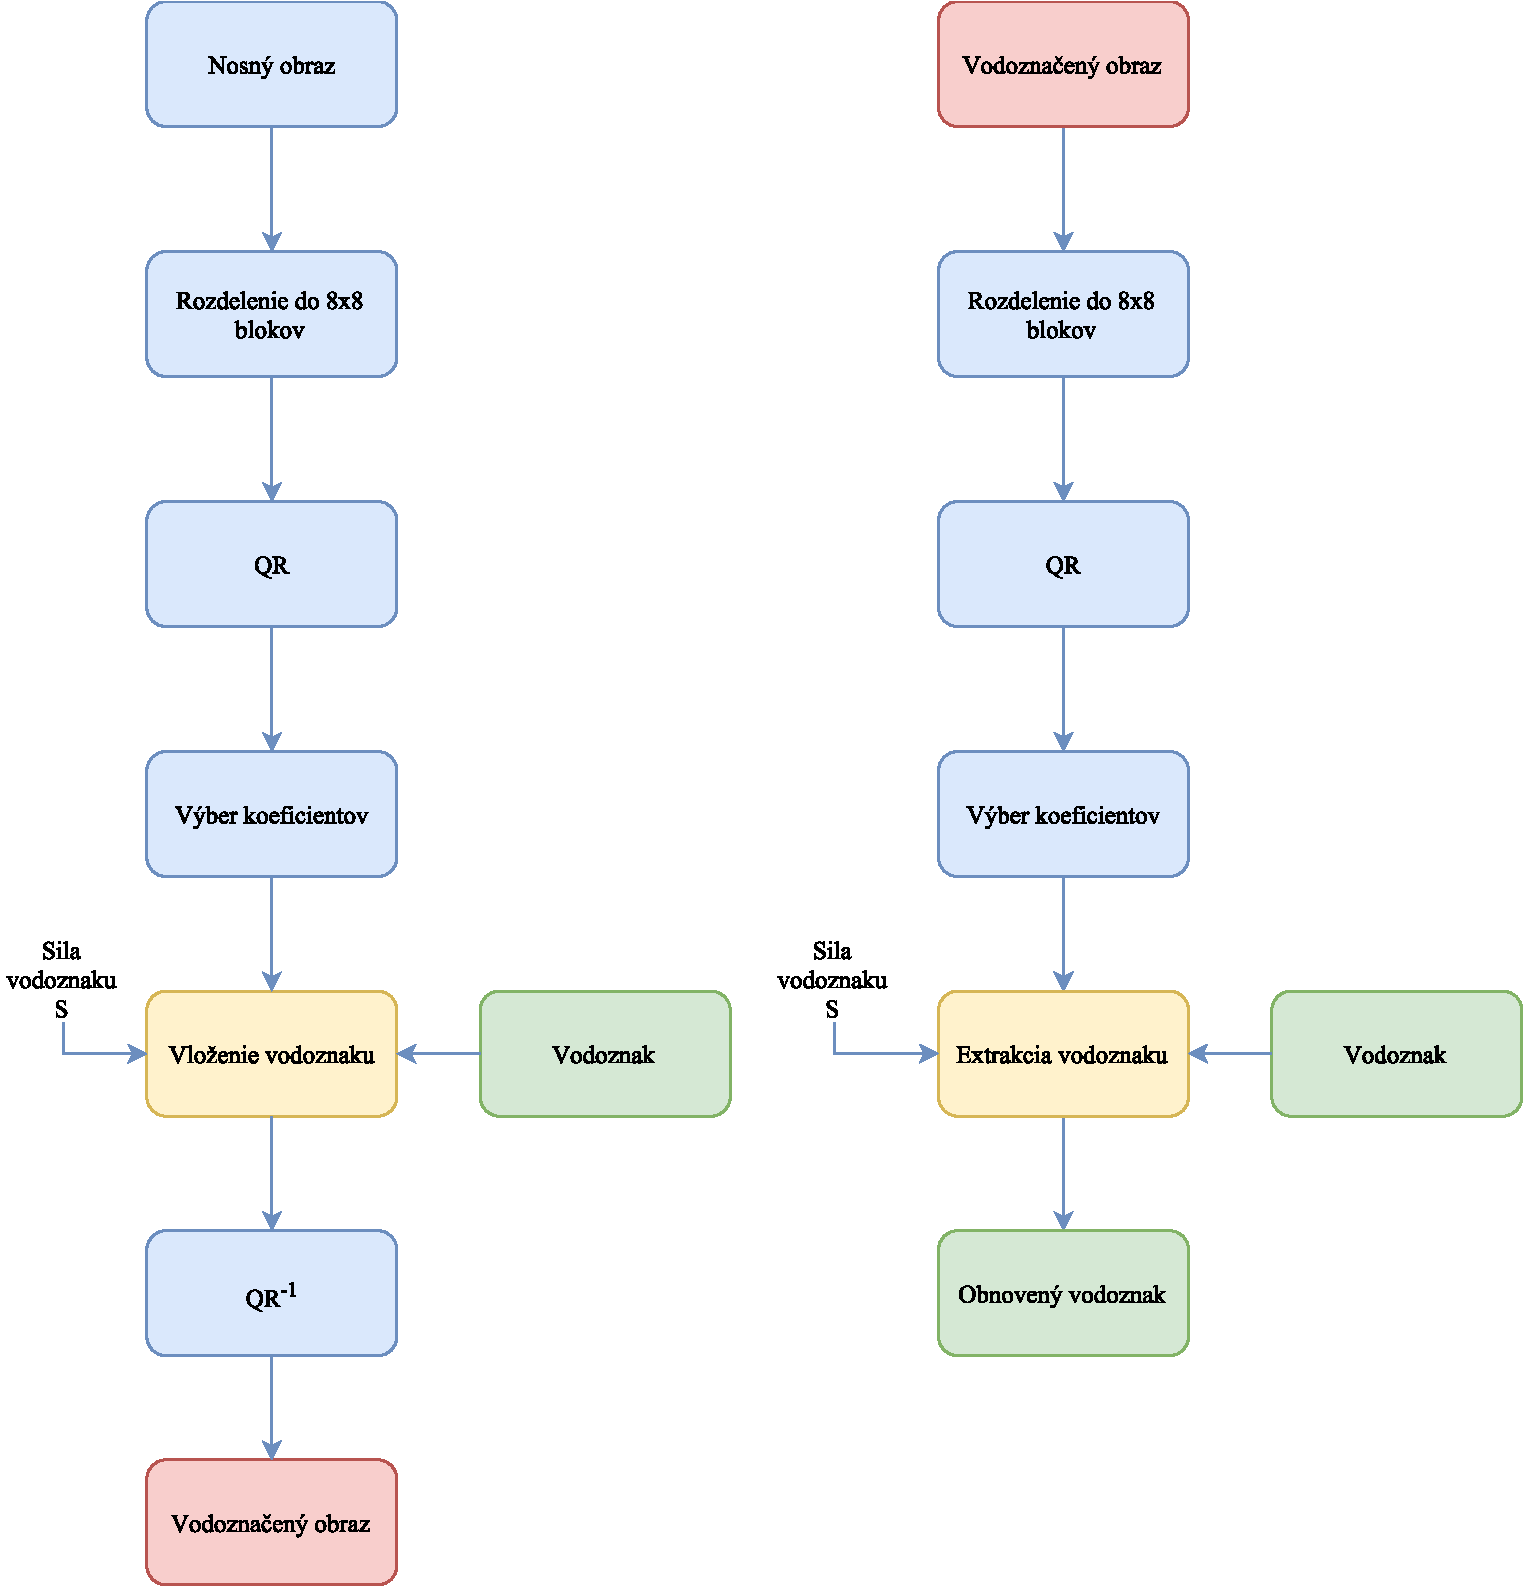
\includegraphics[scale=0.59]{obrazky/embed-extract}
    \caption{Diagram vloženia a extrakcie vodoznaku}
    \label{fig:embed-extract}
\end{figure}

\clearpage
\section{Kapacita}
V~priestorovej doméne je nosný obraz rozdelený do blokov o~rozmeroch $8\times8$ a potom sa do každého z~blokov vloží 8 bitov vodoznaku. Ak budeme uvažovať veľkosť nosného snímku ako $N\times N$, potom maximálna kapacita vkladaného vodoznaku je:

\begin{equation}
\frac{\frac{N\times N}{8\times 8}\times 8}{N \times N} =  0,125(bit/pixel)
\end{equation}

Ako je uvedené v~\cite{QRdecomposition}, kapacita tejto metódy je vyššia ako vo všetkých spomínaných blind metódach, ktoré sú spomenuté v~rovnakom článku. V~tomto článku sa tvrdí, že kapacita tejto metódy je porovnateľná s~non-blind metódami.

\section{Návrh testovania}
Testovanie kvality navrhovanej metódy watermarkingu bude prevádzané prostredníctvom zmeny sily watermarkingu S~a útokov na vodoznačený obraz. Následnou extrakciou vodoznaku môžeme merať odolnosť tejto metódy voči konkrétnym útokom.

K~vyhodnoteniu kvality po prevedení útokov budeme využívať normalizovanú koreláciu (NC) medzi originálnym vodoznakom $\omega$ a extrahovaným vodoznakom $\omega'$.

Kvalita vodoznačeného obrazu bude meraná prostredníctvom pomeru medzi maximálnou možnou energiou signálu a energiou šumu (PSNR). Ako minimálna akceptovateľná hodnota PSNR je považovaná hodnota 37-40dB. Hodnota PSNR sa znižuje so zvyšujúcou sa silou vodoznaku S. Preto musíme nájsť maximálnu hodnotu S~takú, aby nebolo možné pozorovať viditeľné vizuálne zmeny na vodoznačenom obraze. Na druhej strane musí byť hodnota S~dostatočne vysoká na to aby bolo schopné vodoznak extrahovať bez chyby pri nepoužití žiadneho útoku. Vodoznak je extrahovaný bez chyby ak je NC = 1.

Testovať budeme odolnosť vodoznaku voči rotácii obrazu, zmene veľkosti a orezaniu. Použijeme taktiež útoky vo forme vloženia šumu do obrazu, konkrétne Gaussovský šum. Ako ďalšia forma útoku bude použité filtrovanie. Vykonávať budeme mediánové filtrovanie a filtrovanie priemerovaním. Keďže podľa \cite{QRdecomposition} má mať tento systém zvýšenú odolnosť proti JPEG kompresii, tak overíme odolnosť tejto metódy proti rôznym úrovniam JPEG kompresie.

\chapter{Implementácia}
Nasledujúca kapitola sa venuje implementácii navrhovaného algoritmu pre digitálne vodoznačenie obrazu. V~tejto kapitole budú vysvetlené jednotlivé funkcie použité v~programe a taktiež odlišnosti medzi návrhom a implementovaným algoritmom.

Ako už bolo spomenuté v~návrhu v~kapitole \ref{kniznice}, algoritmus je implementovaný v~jazyku C++ s~využitím knižnice ImageMagick. Konkrétne s~využitím objektovo orientovaného API tejto knižnice pre jazyk C++, Magick++. Táto knižnica je postačujúca pre načítanie a uloženie obrazu, ako aj pre transformácie výsledného obrazu, pridanie šumu alebo nastavenie úrovne kompresie. Preto nie je potrebné použiť žiadne ďalšie knižnice.

Časť \ref{impl:load} sa venuje načítaniu jednotlivých pixelov vstupného obrázku do požadovanej dátovej štruktúry tak, aby bola ďalšia práca s~týmito hodnotami čo najjednoduchšia. Nasleduje časť \ref{impl:divide}, ktorá sa zaoberá problémom rozdelenia načítaného obrazu do blokov o~veľkosti $8\times8$ a následného spojenia týchto blokov po prevedení QR rozkladu a vloženia alebo extrakcie vodoznaku. Implementáciu algoritmu pre QR rozklad nájdeme v~\ref{impl:qr}. Proces vkladania a extrakcie vodoznaku a nutné zmeny v~týchto algoritmoch oproti návrhu nájdeme v~\ref{impl:embed-extract}. Nakoniec v~\ref{impl:help} sa nachádza návod na použitie výsledného programu.

\section{Načítanie dát}
\label{impl:load}
Prvým riešeným problémom bolo načítanie intenzít odtieňovej šedej z~obrázku do vhodnej dátovej štruktúry s~ktorou by sa následne pracovalo. Ako dátovú štruktúru je vhodné použiť 2-rozmerné dynamické pole, čo dosiahneme využitím {\tt std::vector}, výsledný nami definovaný dátový typ je {\tt matrix\_t} definovaný ako:

\lstset{language=C++,
    basicstyle=\ttfamily,
    keywordstyle=\color{blue}\ttfamily,
    stringstyle=\color{red}\ttfamily,
    commentstyle=\color{green}\ttfamily,
    morecomment=[l][\color{magenta}]{\#}
}
\begin{lstlisting}
template< typename T > using matrix_t = vector< vector<T> >;
\end{lstlisting}

Obrázok zo súboru načítame pomocou Magick++ metódy {\tt read()}. Táto metóda načíta obrázok do aktuálneho {\tt Magick::Image} objektu. My však potrebujeme iba hodnoty intenzít konkrétnych pixelov. Na tento účel slúži funkcia
\begin{lstlisting}
matrix_t<double> image2matrix(Image &image),
\end{lstlisting}
ktorá uloží hodnoty jednotlivých pixelov do dátového typu {\tt matrix\_t}.

Týmto spôsobom je možné načítať obrázok v~akomkoľvek formáte, ktorý je podporovaný knižnicou ImageMagick. My sme si ako vstupný obrázok vo formáte JPEG zvolili známy obrázok Lena \ref{fig:lena}, ktorý je často používaný pre rôzne úlohy spracovávania obrazu. Tento obrázok má rozlíšenie $512\times512$ pixelov a je v~odtieňoch šedej s~8bitovou hĺbkou. Ako vodoznak používame \ref{fig:watermark} vo formáte PBM s~1bitovou farebnou hĺbkou v~rozlíšení $256\times128$ pixelov. Rozlíšenie vodoznaku je maximálne možné vzhľadom na kapacitu vodoznačiacej metódy pri vstupnom obrázku v~danom rozlíšení.

Pri načítavaní vstupného obrázku metódou {\tt read()} sme objavili, že načítaný obrázok v~odtieňoch šedej nemá iba jeden kanál, ale dva kanály. Jeden kanál obsahuje hodnoty intenzít v~rozsahu $0 - 255$ a druhý v~rozsahu $0-65535$ čo odpovedá rozsahu {\tt QuantumRange} z~Magick++. Ďalšou nečakanou vecou je, že knižnica pracuje s~hodnotou 0 pre čiernu farbu a s~hodnotou 255 pre bielu, čiže opačne ako bolo zamýšľané pri návrhu algoritmov pre vkladanie a extrakciu vodoznaku.

\begin{figure}
    \centering
    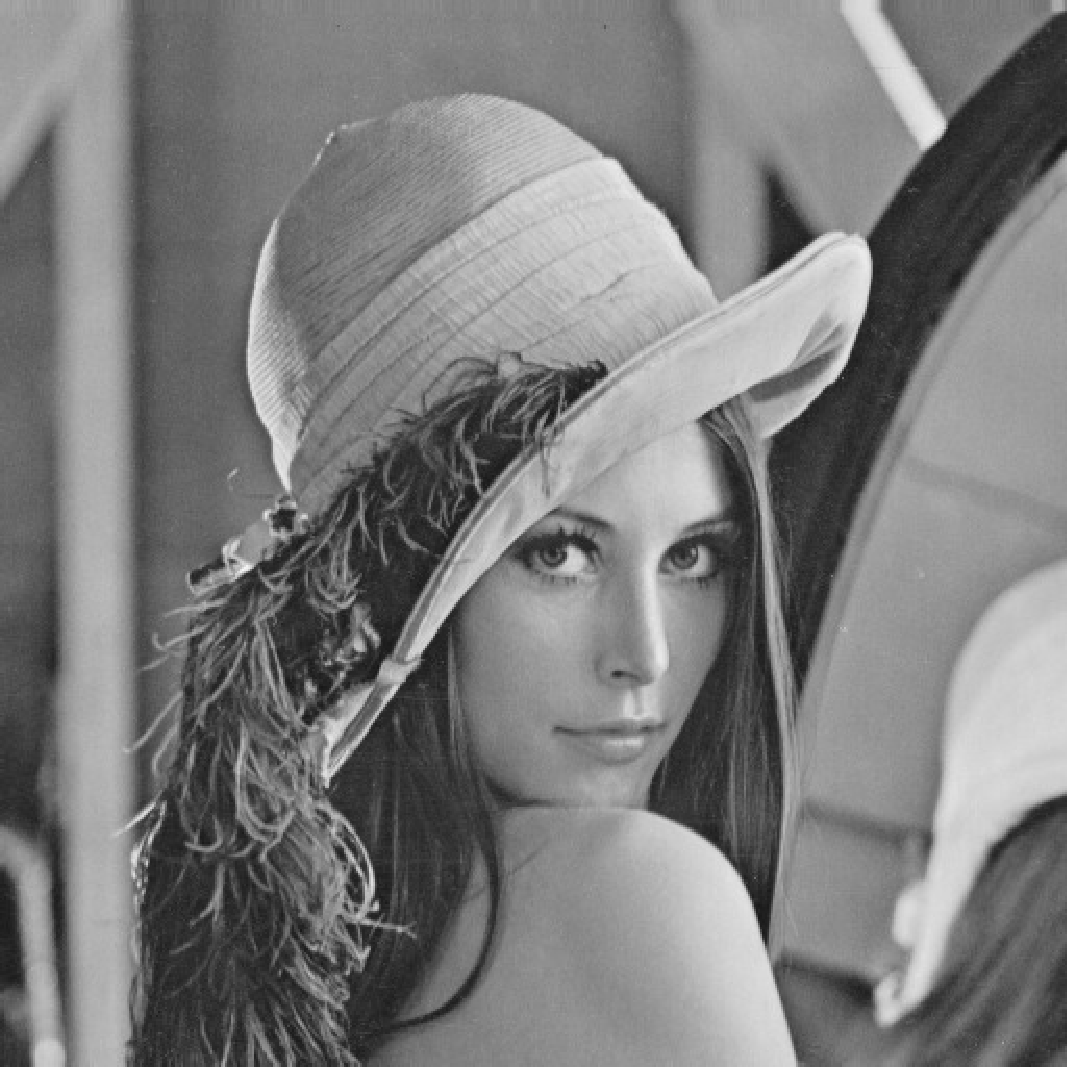
\includegraphics[scale=0.5]{obrazky/lena}
    \caption{Vstupný obrázok - lena.jpg}
    \label{fig:lena}
\end{figure}

\begin{figure}
    \centering
    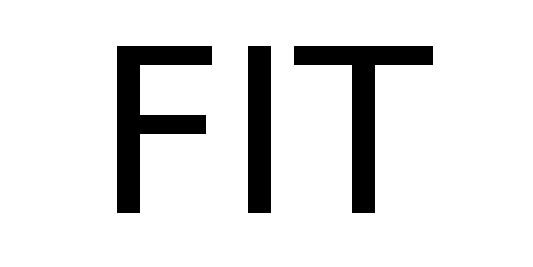
\includegraphics[scale=0.5]{obrazky/fit}
    \caption{Vkladaný vodoznak - fit.pbm}
    \label{fig:watermark}
\end{figure}

\section{Rozdelenie do blokov}
\label{impl:divide}
Kvôli zvýšeniu robustnosti navrhovanej metódy je potrebné načítaný obraz rozdeliť do blokov o~veľkosti $8\time8$ pixelov. Myšlienkou je rozdeliť načítanú maticu intenzít pixelov na skupinu matíc. Na ich uloženie potrebujeme trojdimenzionálne dynamické pole. Ako dátový typ pre uloženie všetkých blokov sme si definovali typ {\tt matrix3d\_t}, ktorý je definovaný nasledovne:
\begin{lstlisting}
template< typename T >
using matrix3d_t = vector< matrix_t<T> >;
\end{lstlisting}

Samotné rozdelenie sa deje pomocou funkcie {\tt get\_blocks()}, ktorej prvým argumentom je matica intenzít pixelov a druhým argumentom je veľkosť bloku. Návratovou hodnotou tejto funkcie je pole všetkých blokov. Táto funkcia je deklarovaná ako:
\begin{lstlisting}
template< typename T >
matrix3d_t<T> get_blocks(const matrix_t<T> &matrix, int n=8)
\end{lstlisting}

Po prevedení QR rozkladu a vložení vodoznaku do nosného obrazu je potrebné bloky naspäť poskladať do výsledného obrazu. Pre zloženie blokov je implementovaná funkcia {\tt concat\_blocks()}, ktorá prechádza všetkými blokmi a spojí ich do výslednej matice typu {\tt matrix\_t}. Deklarácia funkcie je nasledovná:
\begin{lstlisting}
template< typename T >
void concat_blocks(matrix_t<T> &result, matrix3d_t<T> &blocks)
\end{lstlisting}

\section{QR rozklad}
\label{impl:qr}
Táto časť sa venuje algoritmu QR rozkladu\footnote{QR decomposition \url{https://en.wikipedia.org/wiki/QR_decomposition}}, ktorý je základom pre navrhovaný systém vodoznačenia. QR rozklad môžeme dosiahnuť viacerými spôsobmi. Najjednoduchším algoritmom pre vytvorenie QR rozkladu z~matice je {\it Gramov-Schmidtov proces}\footnote{Gram-Schmidt process \url{https://en.wikipedia.org/wiki/Gram–Schmidt_process}}. Medzi ďalšie spôsoby patrí {\it Householderova transformácia}\footnote{Householder transformation \url{https://en.wikipedia.org/wiki/Householder_transformation}} a {\it Givensova rotácia}\footnote{Givens rotation \url{https://en.wikipedia.org/wiki/Givens_rotation}}.

Pre našu implementáciu algoritmu QR rozkladu sme využili {\it Gramov-Schmidtov} proces, konkrétne jeho modifikovanú variantu. Výhodou modifikovaného Gramovho-Schmidtovho procesu je, že je oproti klasickej verzii numericky stabilný\footnote{Numerical stability \url{https://en.wikipedia.org/wiki/Numerical_stability}} 

Tento algoritmus je implementovaný funkciou {\tt gram\_schmidt()}, ktorá zo zadanej matice vytvorí matice $Q$ a $R$ a uloží ich do zoznamov týchto matíc. Deklarácia tejto funkcie je takáto:
\begin{lstlisting}
template< typename T >
void gram_schmidt(matrix_t<T> &matrix, matrix3d_t<T> &q_list,
                  matrix3d_t<T> &r_list)
\end{lstlisting}

Keďže QR rozklad je potrebné vytvoriť nad stĺpcami matice $A$, čiže nad transponovanou maticou $A$, bolo potrebné implementovať funkciu {\tt mat\_transpose()} pre transpozíciu matice dátového typu {\tt matrix\_t}. V~algoritme QR rozkladu je potrebné taktiež vypočítať skalárny súčin vektorov a normalizovaný vektor. Pre skalárny súčin slúži funkcia {\tt dot\_product()} a pre normalizáciu funkcia {\tt normalize()}.
\clearpage
\section{Algoritmus vkladania a extrakcie}
\label{impl:embed-extract}
Po prevedení QR rozkladu nad každým blokom môžeme pristúpiť ku vkladaniu vodoznaku do nosného obrazu. Vodoznaku vkladáme do matice $R$, konkrétne do jej prvého riadku.

Za účelom vkladania vodoznaku do obrazu sme implementovali funkciu {\tt embed()}, ktorej deklarácia je takáto:
\begin{lstlisting}
template< typename T >
void embed(matrix_t<T> &matrix, vector<T> &watermark,
           int strength, int iteration, int size=8)
\end{lstlisting}

Keďže hodnoty pre čierny a biely pixel pri použití knižnice ImageMagick sú opačné ako sme očakávali, museli sme upraviť aj vzorec \ref{embed} pre vloženie vodoznaku do obrazu. Upraviť bolo potrebné tiež hodnotu vodoznaku, pretože skúmame hodnotu konkrétneho pixelu, ktorá nadobúda hodnoty buď 0 alebo 255. Výsledný vzorec použitý pri implementácii je nasledovný:

\begin{equation} \label{embed-mod}
\left \{
  \begin{tabular}{ll}
  $C' = C - (C\mod S) + T_1 \qquad$ & $if \quad \omega = 255$ \\
  $C' = C - (C\mod S) + T_2 \qquad$ & $if \quad \omega = 0$
  \end{tabular}
\right.
\end{equation}

Pre extrakciu vodoznaku je implementovaná funkcia {\tt extract()} deklarovaná ako:
\begin{lstlisting}
template< typename T >
void extract(matrix_t<T> &matrix, vector<T> &watermark,
             int strength, int size=8)
\end{lstlisting}

Vzorec pre extrakciu vodoznaku \ref{extract} bolo potrebné upraviť podobne ako vzorec pre vkladanie vodoznaku. Dôvodom je taktiež to, že pracujeme s~hodnotami 0 a 255. Upravený vzorec je:

\begin{equation} \label{extract-mod}
\left \{
  \begin{tabular}{ll}
  $\omega' = 255,\qquad$ & $if (C''\mod S) > \frac{T_1+T_2}{2}$ \\
  $\omega' = 0,\qquad$  & $if (C''\mod S) < \frac{T_1+T_2}{2}$
  \end{tabular}
\right.
\end{equation}

\section{Použitie programu}
\label{impl:help}
Výsledný program s~názvom {\tt watermarking} dokáže vložiť zadaný vodoznak do obrázku v~jednom z~vyše 200 podporovaných obrazových formátov, ktoré sú podporované knižnicou ImageMagick. Program dokáže extrahovať vodoznak z~obrázku a porovnať ho s~referenčným vodoznakom. Umožnené je tiež spustenie programu s~útokmi na vodoznačený obraz, ktoré sa využijú v~kapitole \ref{testy}.

Prepínače sú nasledovné:
\begin{itemize}
\item {\verb|--help|} - zobrazí nápovedu k~programu
\item {\verb|--input FILE|} - určenie vstupného obrázku
\item {\verb|--output FILE|} - určenie kam sa uloží vodoznačený obraz
\item {\verb|--wm-input FILE|} - názov súboru obsahujúci vodoznak
\item {\verb|--wm-output FILE|} - názov súboru, kam sa má uložiť extrahovaný vodoznak
\item {\verb|--strength NUMBER|} - nastavenie úrovne sily vodoznačiacej metódy
\item {\verb|--quality NUMBER<0-100>|} - nastavenie úrovne kompresie výstupného vodoznačeného obrazu
\item {\verb|--embed|} - vkladanie vodoznaku
\item {\verb|--extract|} - extrakcia vodoznaku
\item {\verb|--attack|} - prevedenie série útokov na vodoznačený obraz
\item {\verb|--statistics|} - zobrazenie NC extrahovaného a pôvodného vodoznaku a PSNR medzi originálnym a vodoznačeným obrazom 
\end{itemize}

Jediným povinným argumentom sú prepínače \verb|--input| a \verb|--wm-input|, ktorými špecifikujeme vstupné dáta. Pri neuvedení prepínačov \verb|--embed| a \verb|--extract| sa prevedie vloženie a aj následná extrakcia vodoznaku. Použitie prepínača \verb|--statistics| je podmienené extrakciou vodoznaku, čiže je potrebné použiť prepínač \verb|--extract| alebo nepoužiť žiaden z~prepínačov \verb|--embed, --extract|.


\chapter{Testy a výsledky} \label{testy}
Jednou z~hlavných vlastností vodoznaku okrem jeho kapacity a nevnímateľnosti je jeho robustnosť. V~prípade použitia vodoznaku pre ochranu autorských práv je táto vlastnosť nesmierne dôležitá. Môžeme mať vodoznačiacu metódu, ktorá má vysokú kapacitu a ktorá dokáže do obrazu vložiť vodoznak, ktorý je ľudským okom nepostrehnuteľný, ale ak je tento vodoznak možné poškodiť bežným spracovaním obrazu natoľko, že nie je čitateľný, tak takáto metóda nebude vhodná napríklad pre ochranu autorských práv.

Práve preto sa táto kapitola venuje testovaniu implementovanej metódy watermarkingu. Pre účely testovania program umožňuje použiť prepínač \verb|--attack|, ktorý vykoná všetky útoky zobrazené v~nasledujúcich podkapitolách.
Testované budú rôzne metódy vylepšenia obrázku \ref{enhance} a vkladania šumu \ref{noise}. V~rámci overovania odolnosti taktiež otestujeme tento algoritmus voči zaostreniu obrazu a ekvalizácii histogramu. Následne vyskúšame robustnosť algoritmu proti transformáciám ako sú rotácia alebo zmena veľkosti \ref{transform}. Na záver podrobíme testovaný obrázok JPEG kompresii \ref{compress}.

\section{Zvolenie sily vodoznaku}
Skôr ako sa pustíme do testovania robustnosti tejto metódy musím nájsť vhodnú hodnotu pre silu vodoznačenia. Pre nájdenie vhodnej hodnoty sily vodoznaku $S$ je nutné splniť dve podmienky.

Prvou podmienkou je, že po vložení vodoznaku musí byť možné bez chyby vodoznak z~obrázku extrahovať. K~porovnaniu vloženého a extrahovaného vodoznaku nám slúži normalizovaná korelácia $NC$, ak je vodoznak extrahovaný bez chyby, tak $NC = 1$.

Druhou podmienkou je neviditeľnosť vodoznaku. So zvyšujúcou sa silou vodoznaku $S$ rastie počet viditeľných zmien v~obraze, preto musíme zvoliť silu vodoznaku tak, aby bola sila vodoznaku čo najvyššia a aby bol vodoznak neviditeľný. K~tomuto účelu slúži pomer medzi energiou signálu a energiou šumu $PSNR$. Vo väčšine článkov sa dozvedáme, že minimálna akceptovateľná hodnota $PSNR$ je 37-40dB.

Na základe vyššie uvedených testov rôznych úrovní sily vodoznaku sme zvolil hodnotu $S=24$, pretože pri hodnote $S=26$ s~$PSNR=37,39dB$ už boli jasne zreteľné zmeny v~obraze. 
\clearpage

\begin{table}[ht]
\centering
\label{wm-strength}
\begin{tabular}{lll}
\hline
\multicolumn{1}{c}{\textbf{Sila vodoznaku}} & \multicolumn{1}{c}{\textbf{NC}} & \multicolumn{1}{c}{\textbf{PSNR}} \\ \hline
1                              & 1                               & 62,95 \\
5                              & 1                               & 51,64 \\
10                             & 1                               & 45,91 \\
15                             & 1                               & 41,99 \\
20                             & 1                               & 39,43 \\
22                             & 1                               & 38,94 \\
24                             & 1                               & 37,86 \\
26                             & 1                               & 37,39 \\ \hline
\end{tabular}
\caption{Zvolenie sily vodoznaku}
\end{table}

\section{Vloženie šumu} \label{noise}
V~nasledujúcej tabuľke \ref{noise-table} sú zobrazené útoky vložením šumu do vodoznačeného obrazu. Môžeme si všimnúť, že náš algoritmus vodoznačenia sa dokáže vysporiadať jedine s~rovnomerným šumom. Pri ostatných druhoch šumu považujeme vodoznak za nerozoznateľný.
\begin{table}[h]
\centering
\label{noise-table}
\begin{tabular}{llcc}
\hline
\multicolumn{1}{c}{\textbf{Typ útoku}} & \multicolumn{1}{c}{\textbf{NC}} & \multicolumn{1}{c}{\textbf{Vodoznačený obraz}} & \multicolumn{1}{c}{\textbf{Extrahovaný vodoznak}} \\ \hline
Gaussovský šum                         & 0.002 & 
\begin{minipage}[c]{.1\textwidth}
\ 
  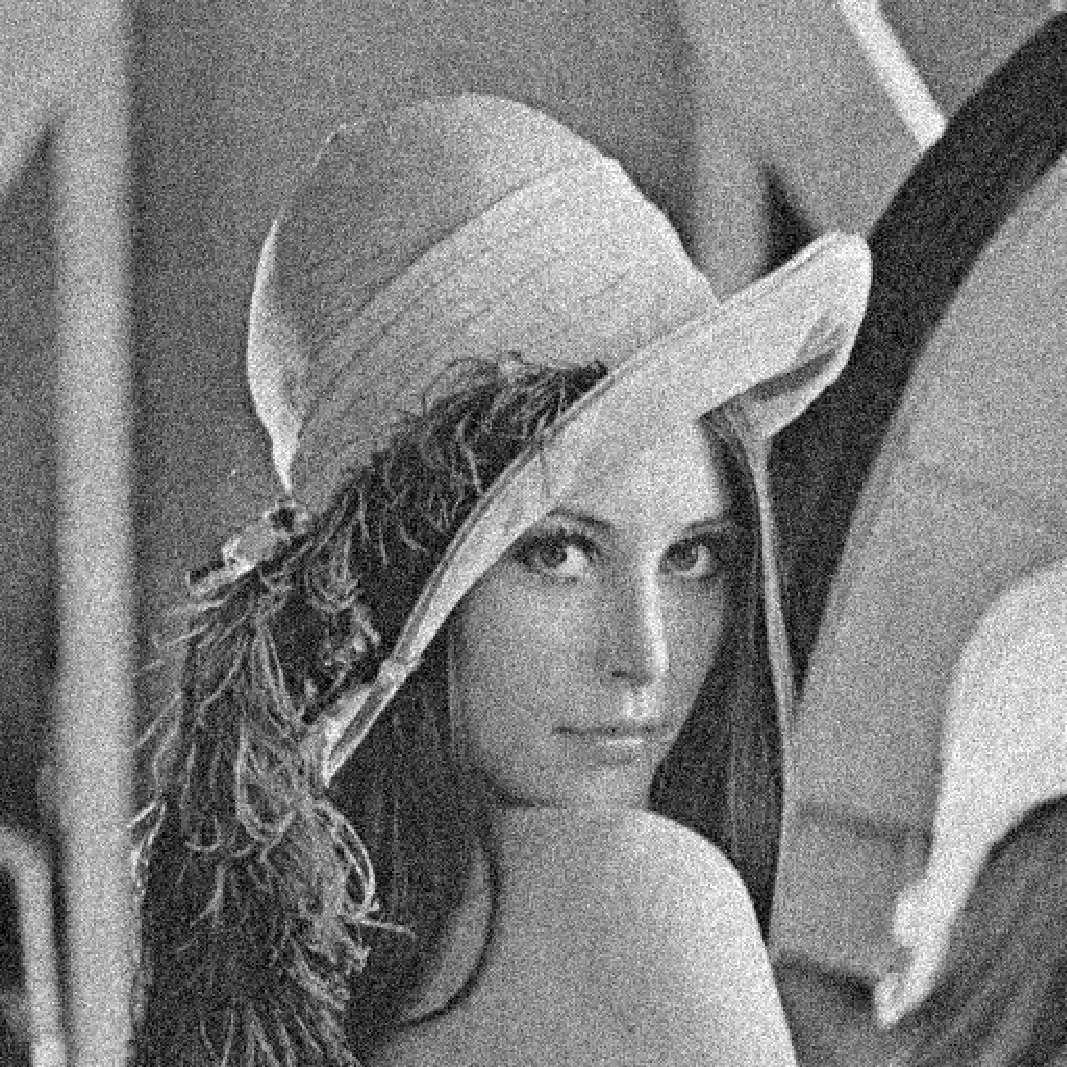
\includegraphics[scale=0.1]{obrazky/GaussianNoise}
\end{minipage} & 
\begin{minipage}[c]{.15\textwidth}
\ 
  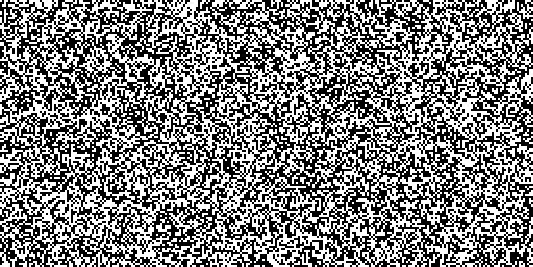
\includegraphics[scale=0.25]{obrazky/GaussianNoise-wm}
\end{minipage}  \\
Rovnomerný šum                         &  1 & 
\begin{minipage}[c]{.1\textwidth}
\ 
  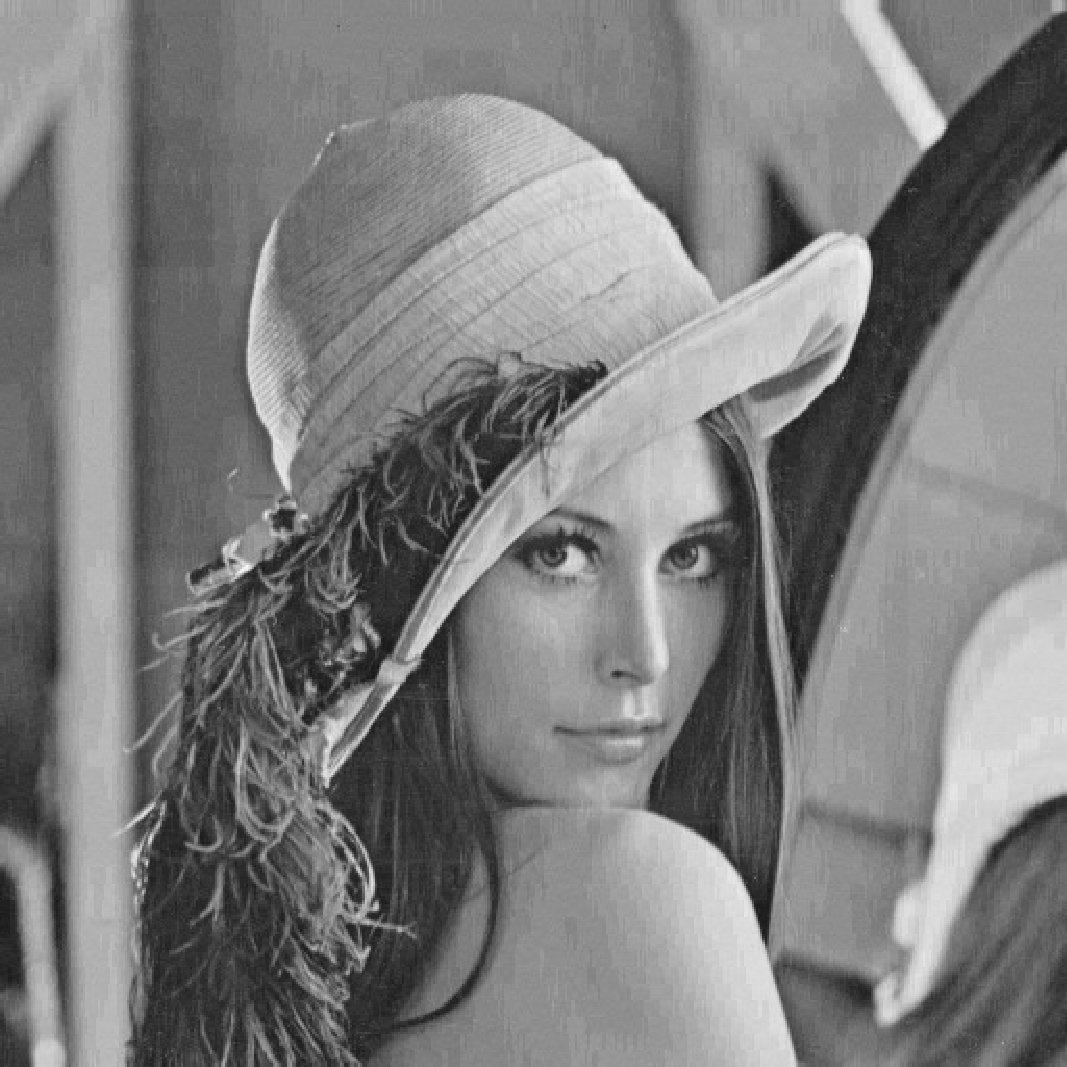
\includegraphics[scale=0.1]{obrazky/UniformNoise}
\end{minipage} & 
\begin{minipage}[c]{.15\textwidth}
\ 
  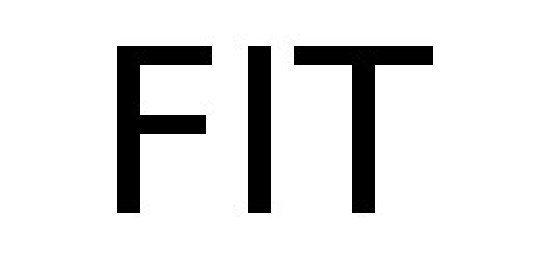
\includegraphics[scale=0.25]{obrazky/UniformNoise-wm}
\end{minipage}  \\
Laplaceov šum                          & 0.002 & 
\begin{minipage}[c]{.1\textwidth}
\ 
  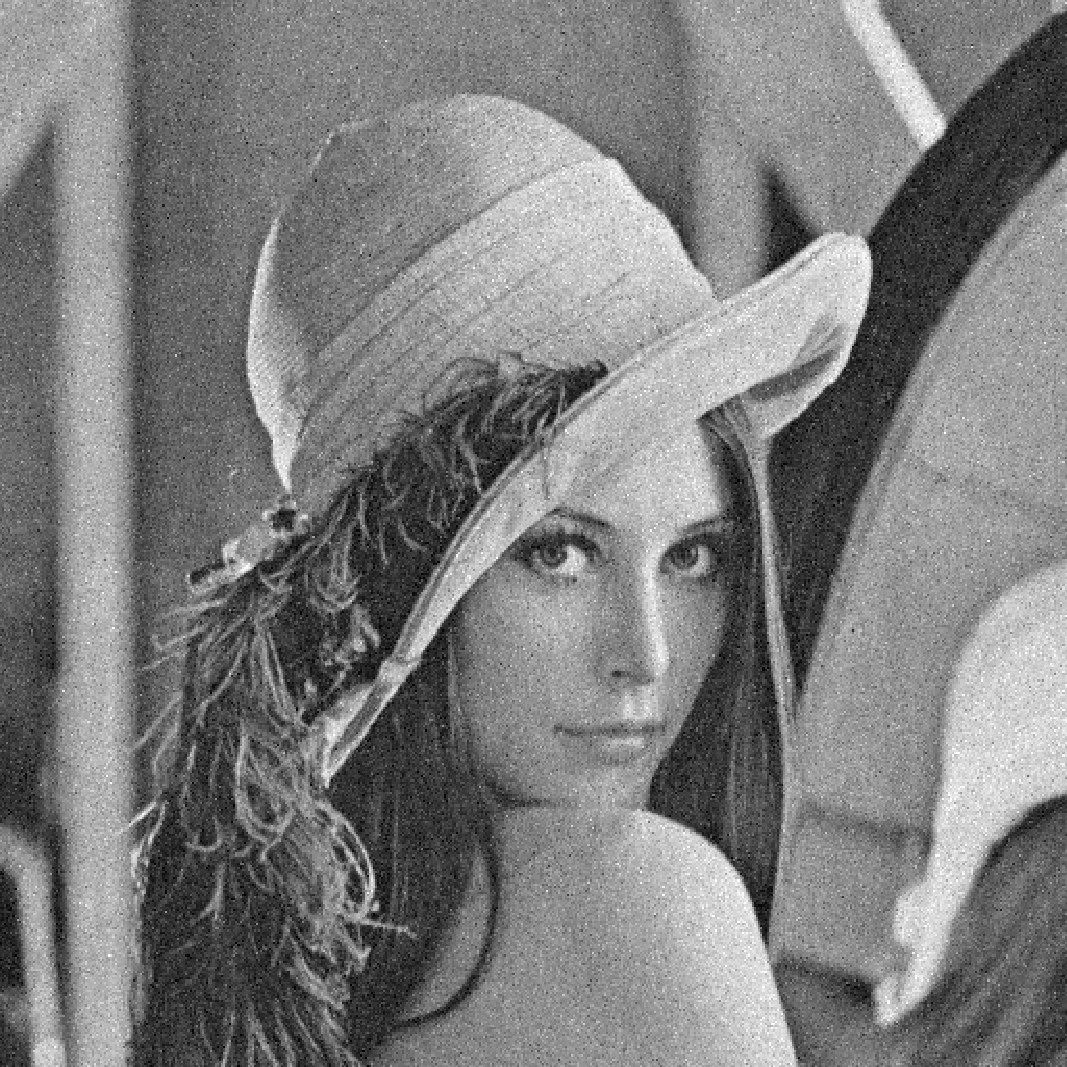
\includegraphics[scale=0.1]{obrazky/LaplacianNoise}
\end{minipage} & 
\begin{minipage}[c]{.15\textwidth}
\ 
  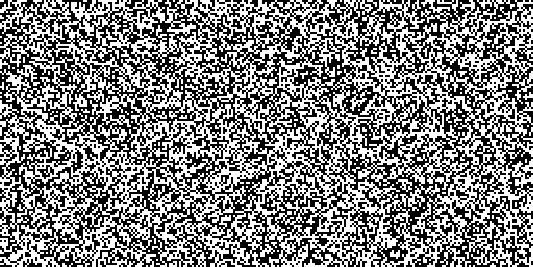
\includegraphics[scale=0.25]{obrazky/LaplacianNoise-wm}
\end{minipage}  \\
Poissonov šum                          & 0.002 & 
\begin{minipage}[c]{.1\textwidth}
\ 
  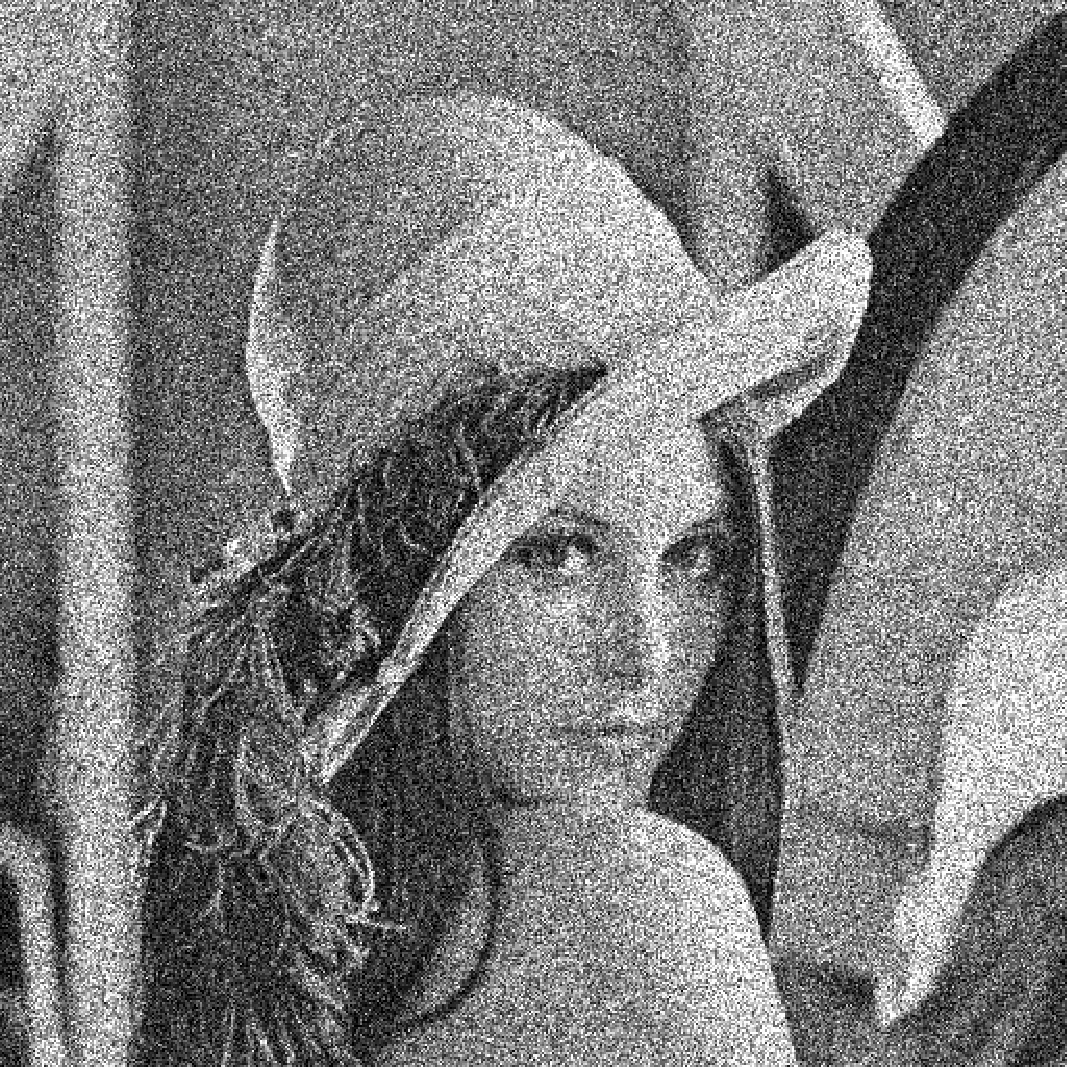
\includegraphics[scale=0.1]{obrazky/PoissonNoise}
\end{minipage} & 
\begin{minipage}[c]{.15\textwidth}
\ 
  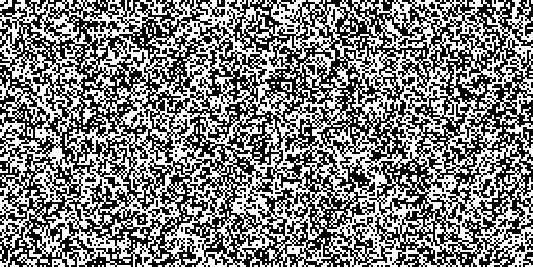
\includegraphics[scale=0.25]{obrazky/PoissonNoise-wm}
\end{minipage}  \\ \hline
\end{tabular}
\caption{Útoky vložením šumu}
\end{table}

\section{Vylepšenie obrazu} \label{enhance}
Tabuľka \ref{enhance-table} zobrazuje vykonané vylepšenia obrazu a ich dopad na vložený vodoznak. Ako môžeme vidieť, algoritmus pre vkladanie vodoznaku je robustnejší proti rôznym metódam vyhladzovania obrazu ako proti útokom, ktoré do obrazu vložia šum.

Z~dát z~tabuľky vidíme, že najväčšiu robustnosť má algoritmus proti mediánovému filtru, kde sme schopní extrahovať nezmenený vodoznak. Pri odstránení šumu, vyhladení a zaostrení je to už horšie, no stále sme schopní rozoznať vodoznak. Z~týchto útokov sa ukázal ako najtvrdší útok ekvalizovaním histogramu, pri ktorom môžeme považovať vodoznak za zničený.
\begin{table}[h]
\centering
\label{enhance-table}
\begin{tabular}{llcc}
\hline
\multicolumn{1}{c}{\textbf{Typ útoku}} & \multicolumn{1}{c}{\textbf{NC}} & \multicolumn{1}{c}{\textbf{Vodoznačený obraz}} & \multicolumn{1}{c}{\textbf{Extrahovaný vodoznak}} \\ \hline
Rozmazanie                             & 0.287 &
\begin{minipage}[c]{.1\textwidth}
\ 
  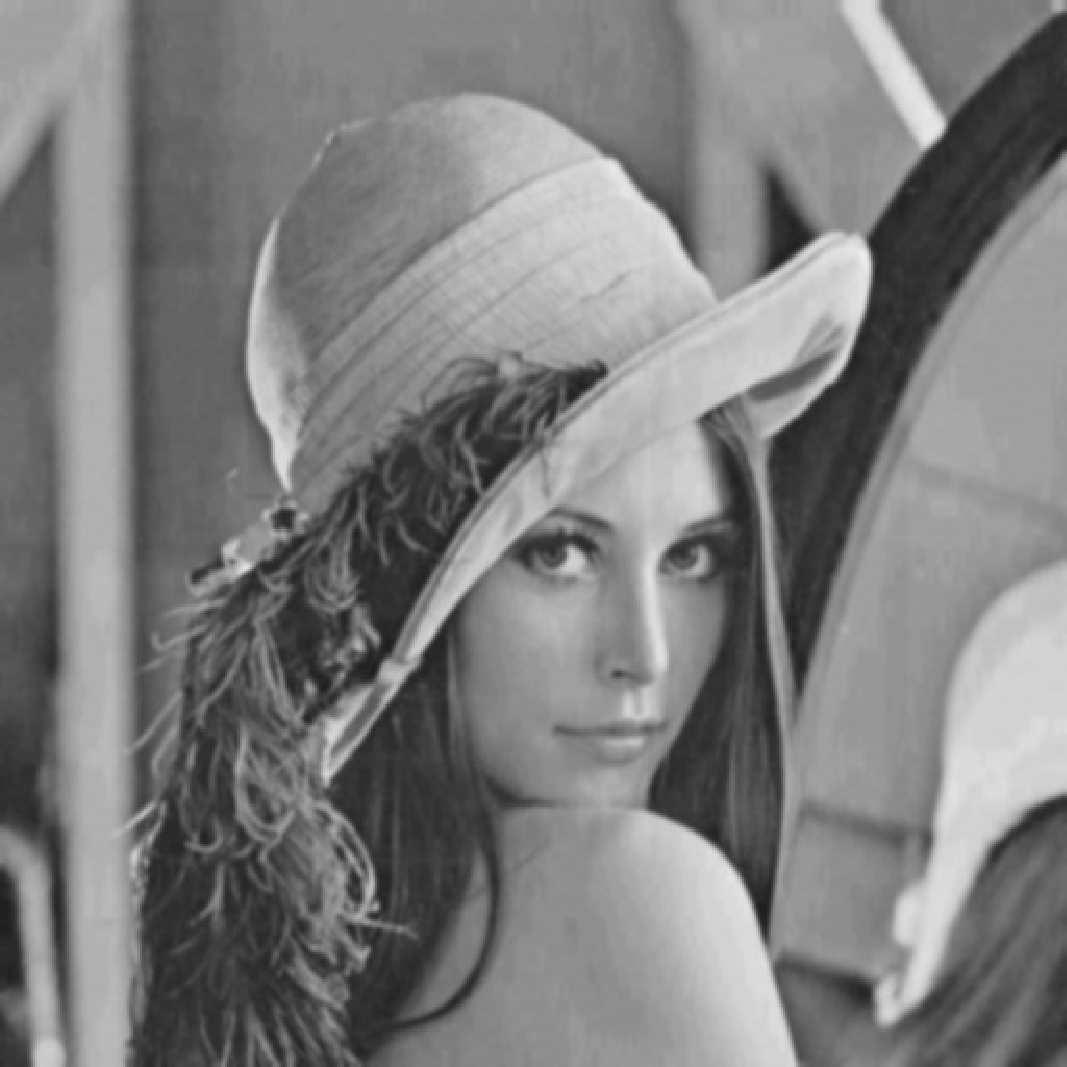
\includegraphics[scale=0.1]{obrazky/blur}
\end{minipage} &
\begin{minipage}[c]{.15\textwidth}
\ 
  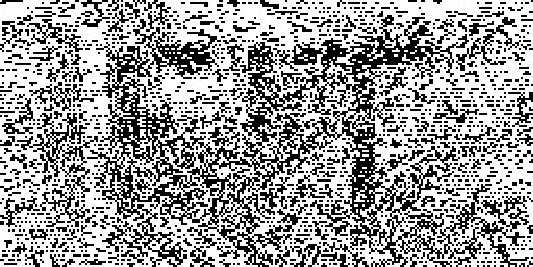
\includegraphics[scale=0.25]{obrazky/blur-wm}
\end{minipage} \\
Gaussovské rozostrenie                 & 0.281 &
\begin{minipage}[c]{.1\textwidth}
\ 
  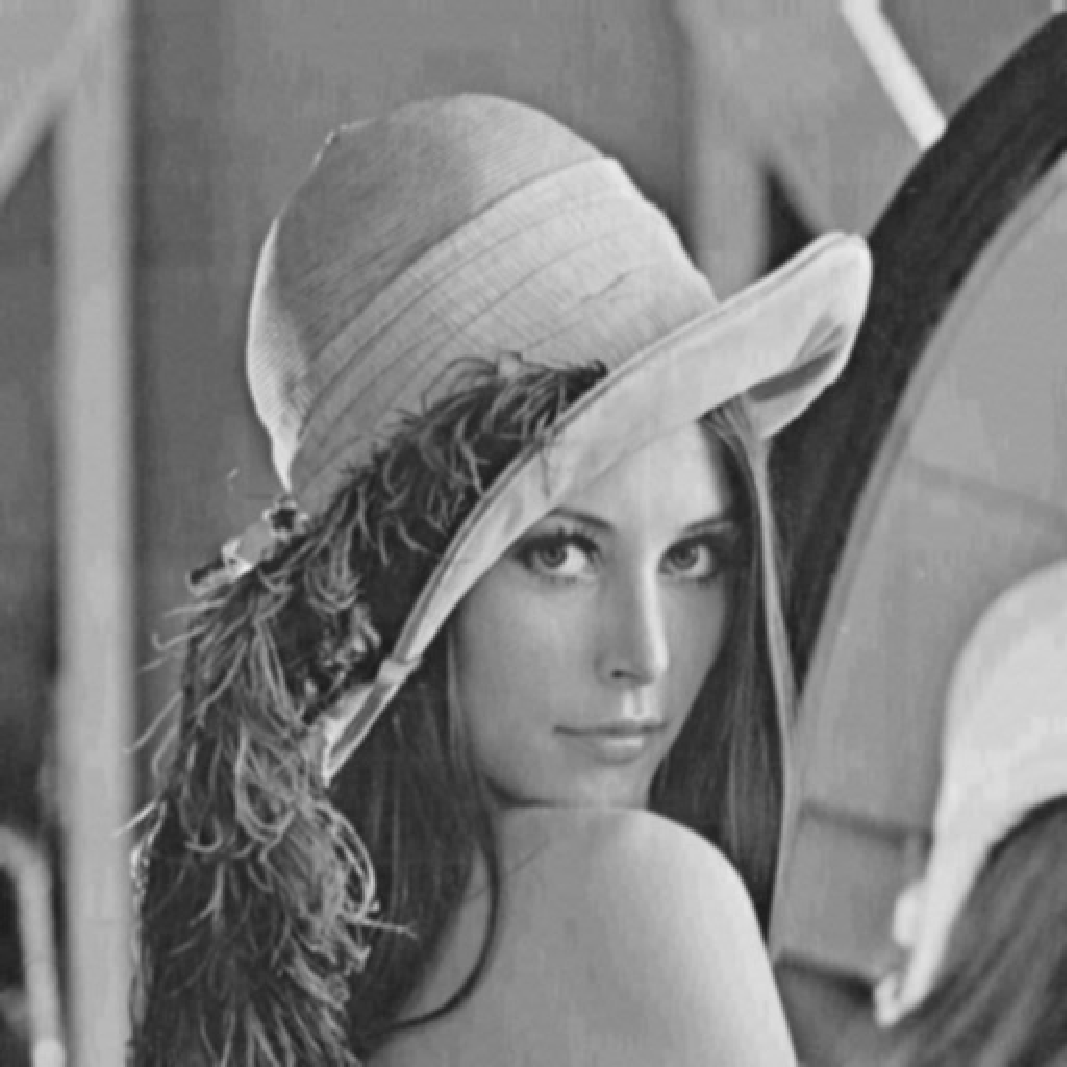
\includegraphics[scale=0.1]{obrazky/gaussianBlur}
\end{minipage} &
\begin{minipage}[c]{.15\textwidth}
\ 
  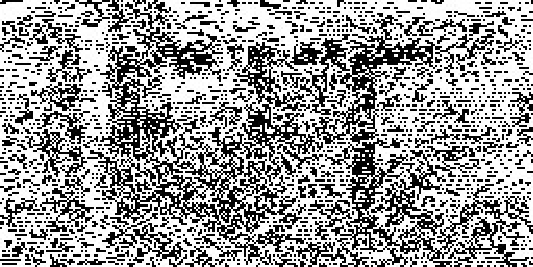
\includegraphics[scale=0.25]{obrazky/gaussianBlur-wm}
\end{minipage} \\
Mediánový filter                       &  1 &
\begin{minipage}[c]{.1\textwidth}
\ 
  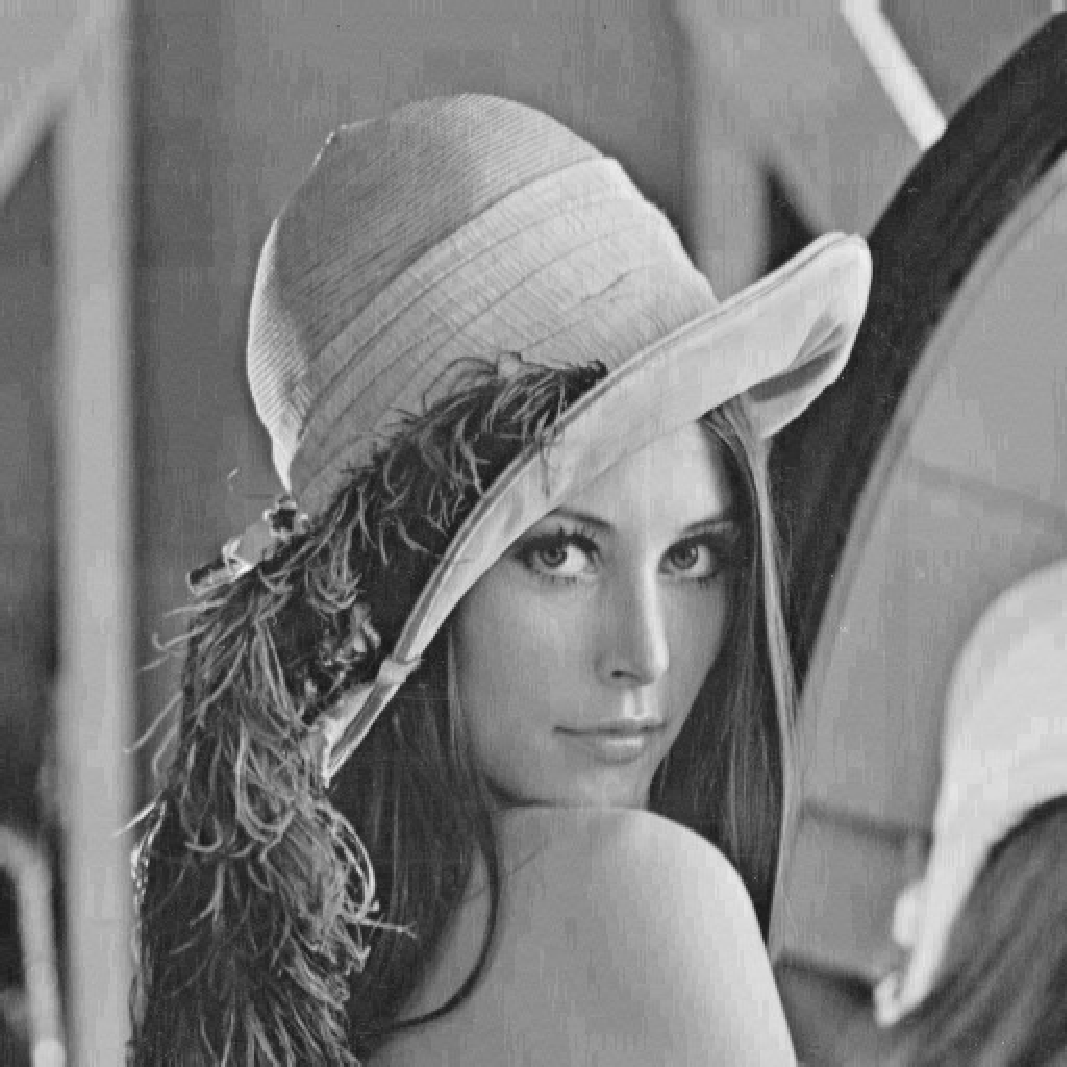
\includegraphics[scale=0.1]{obrazky/medianFilter}
\end{minipage} &
\begin{minipage}[c]{.15\textwidth}
\ 
  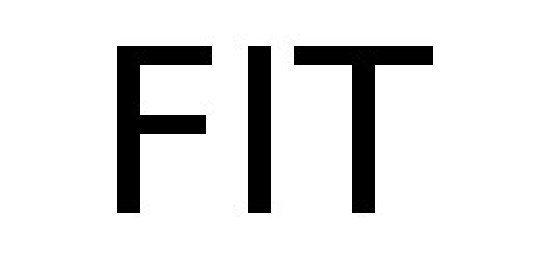
\includegraphics[scale=0.25]{obrazky/medianFilter-wm}
\end{minipage} \\
Filtrovanie priemerovaním              & 0.195 &
\begin{minipage}[c]{.1\textwidth}
\ 
  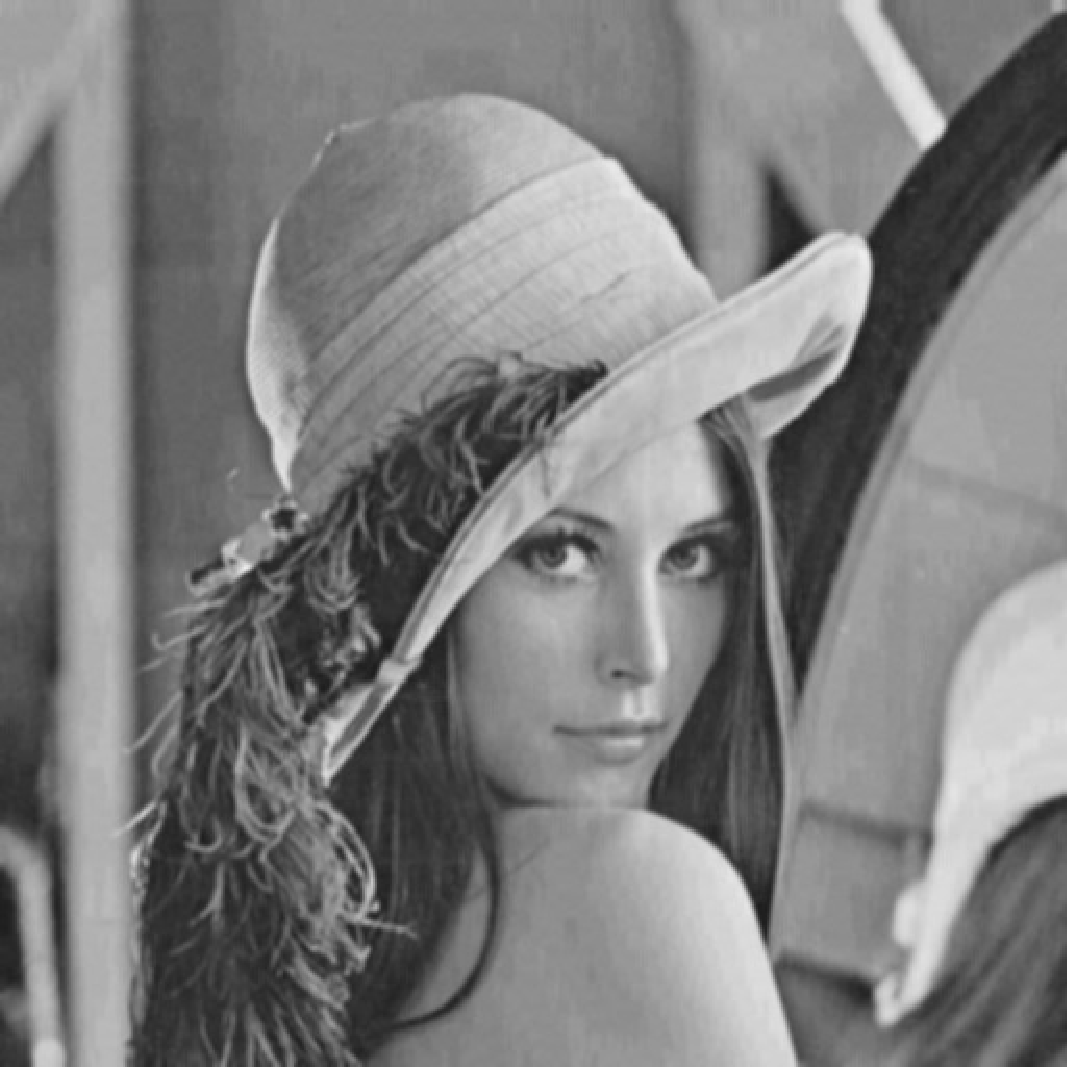
\includegraphics[scale=0.1]{obrazky/averageFilter}
\end{minipage} &
\begin{minipage}[c]{.15\textwidth}
\ 
  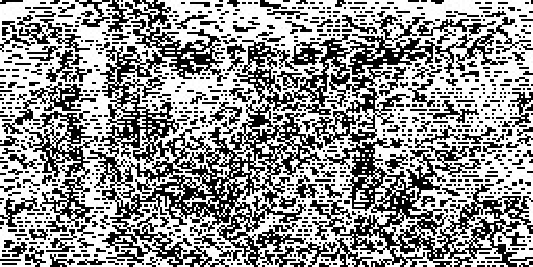
\includegraphics[scale=0.25]{obrazky/averageFilter-wm}
\end{minipage} \\
Odstránenie šumu                       & 0.590 &
\begin{minipage}[c]{.1\textwidth}
\ 
  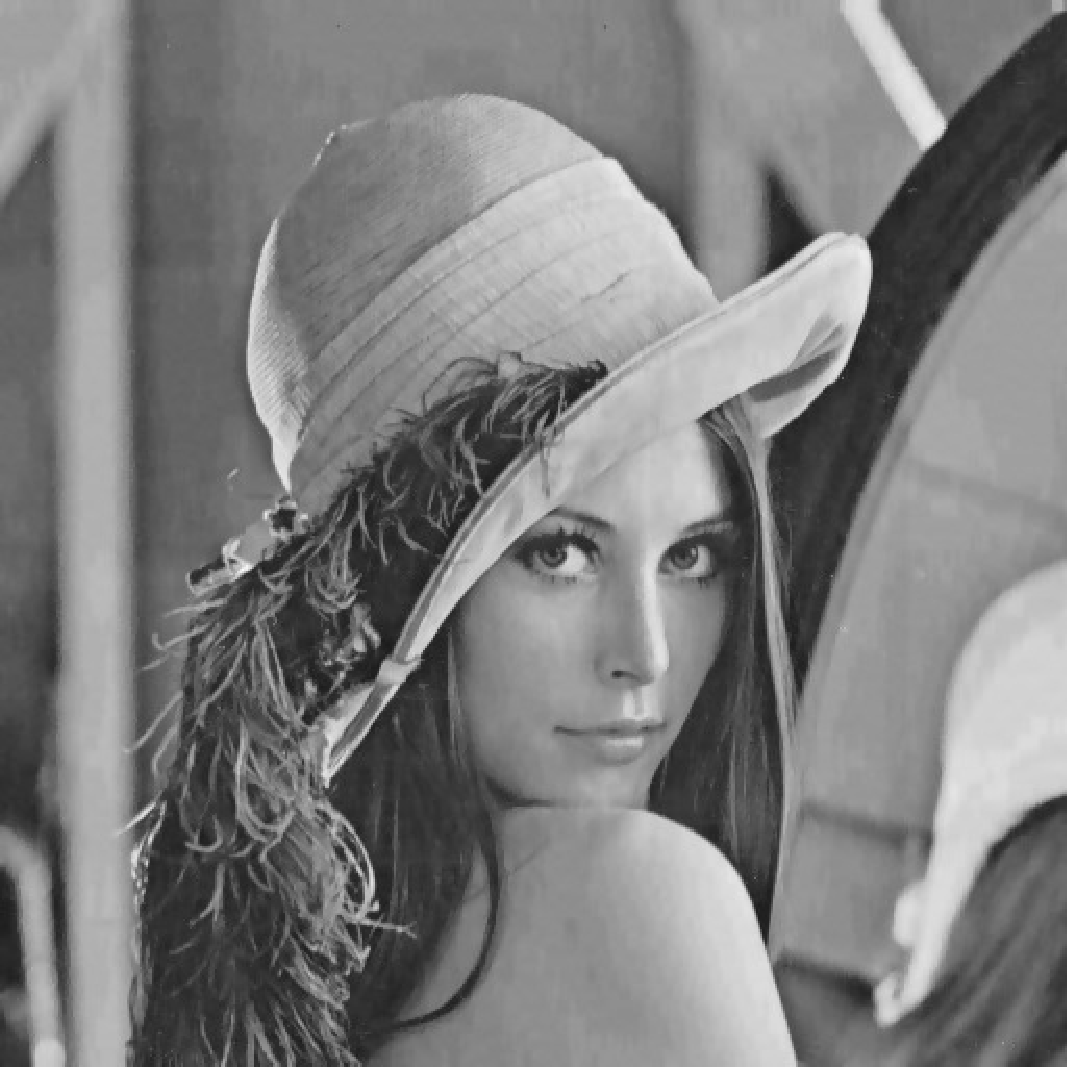
\includegraphics[scale=0.1]{obrazky/enhance}
\end{minipage} &
\begin{minipage}[c]{.15\textwidth}
\ 
  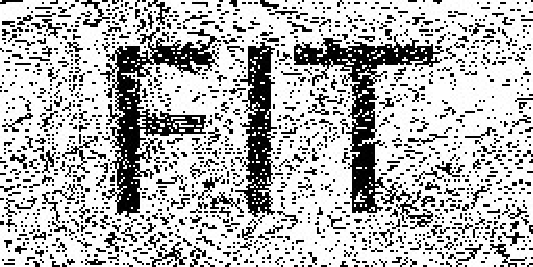
\includegraphics[scale=0.25]{obrazky/enhance-wm}
\end{minipage} \\
Vyhladenie                             & 0.449 &
\begin{minipage}[c]{.1\textwidth}
\ 
  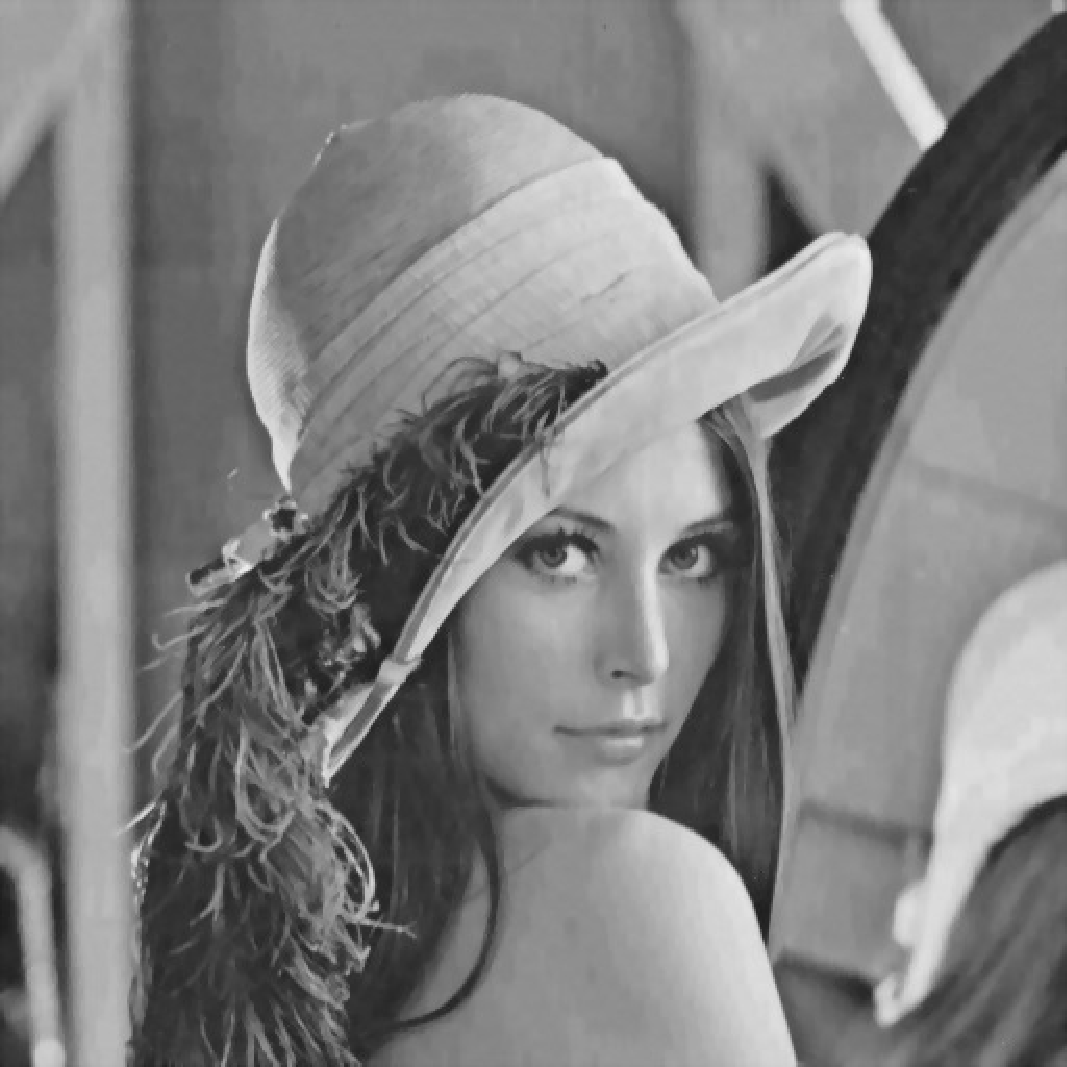
\includegraphics[scale=0.1]{obrazky/despeckle}
\end{minipage} &
\begin{minipage}[c]{.15\textwidth}
\ 
  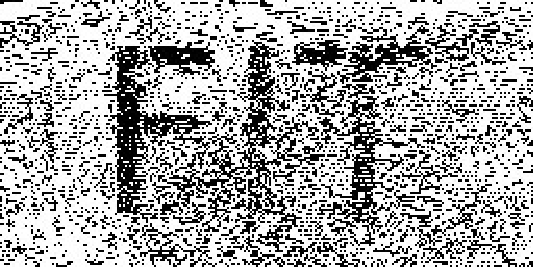
\includegraphics[scale=0.25]{obrazky/despeckle-wm}
\end{minipage} \\
Zaostrenie                             & 0.408 &
\begin{minipage}[c]{.1\textwidth}
\ 
  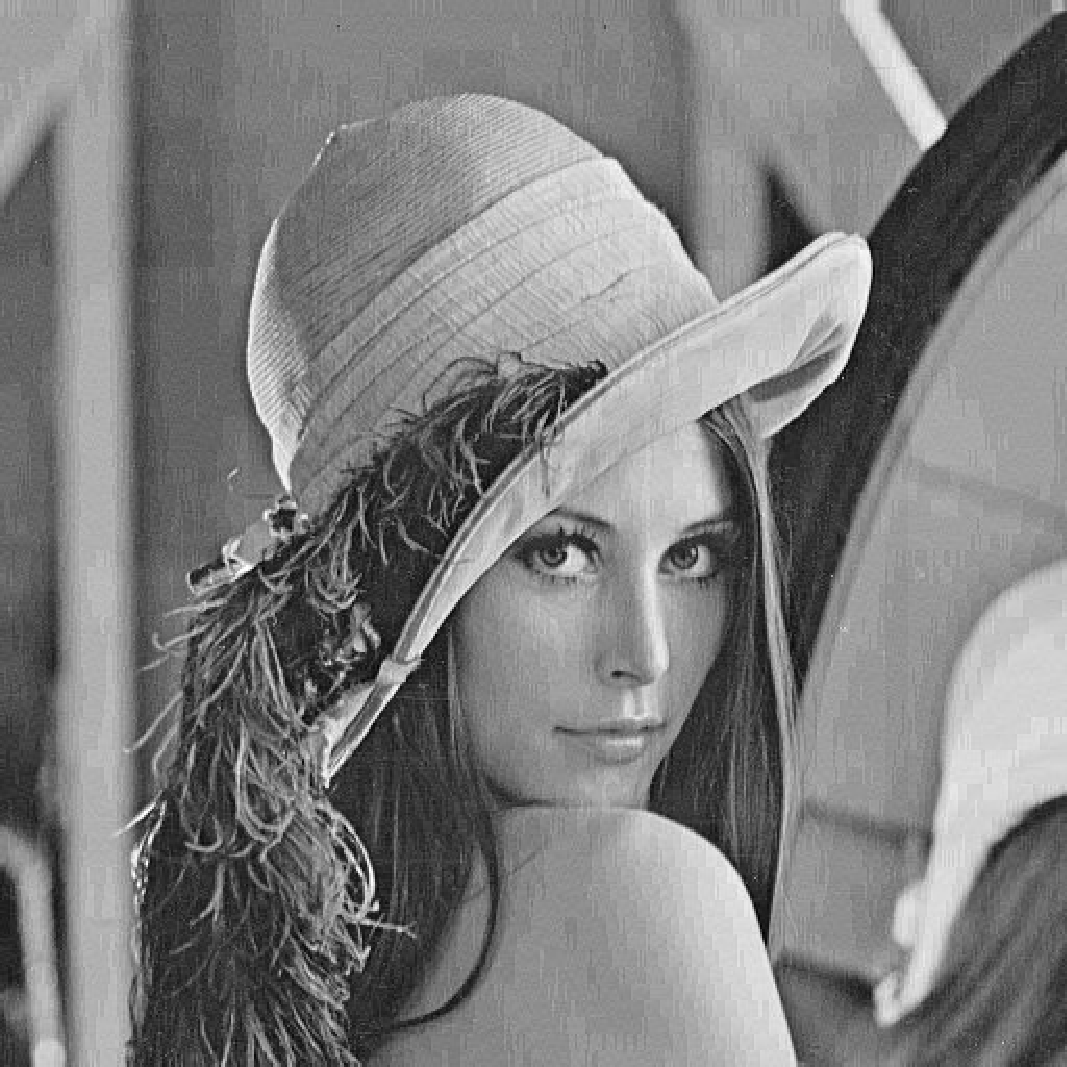
\includegraphics[scale=0.1]{obrazky/sharpen}
\end{minipage} &
\begin{minipage}[c]{.15\textwidth}
\ 
  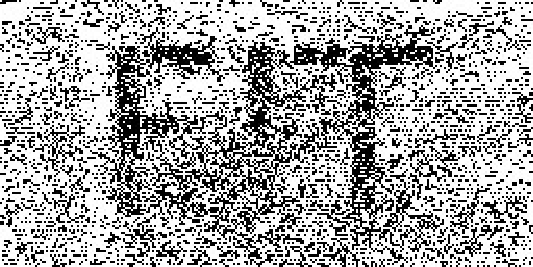
\includegraphics[scale=0.25]{obrazky/sharpen-wm}
\end{minipage} \\
Ekvalizácia histogramu                 & 0.031 &
\begin{minipage}[c]{.1\textwidth}
\ 
  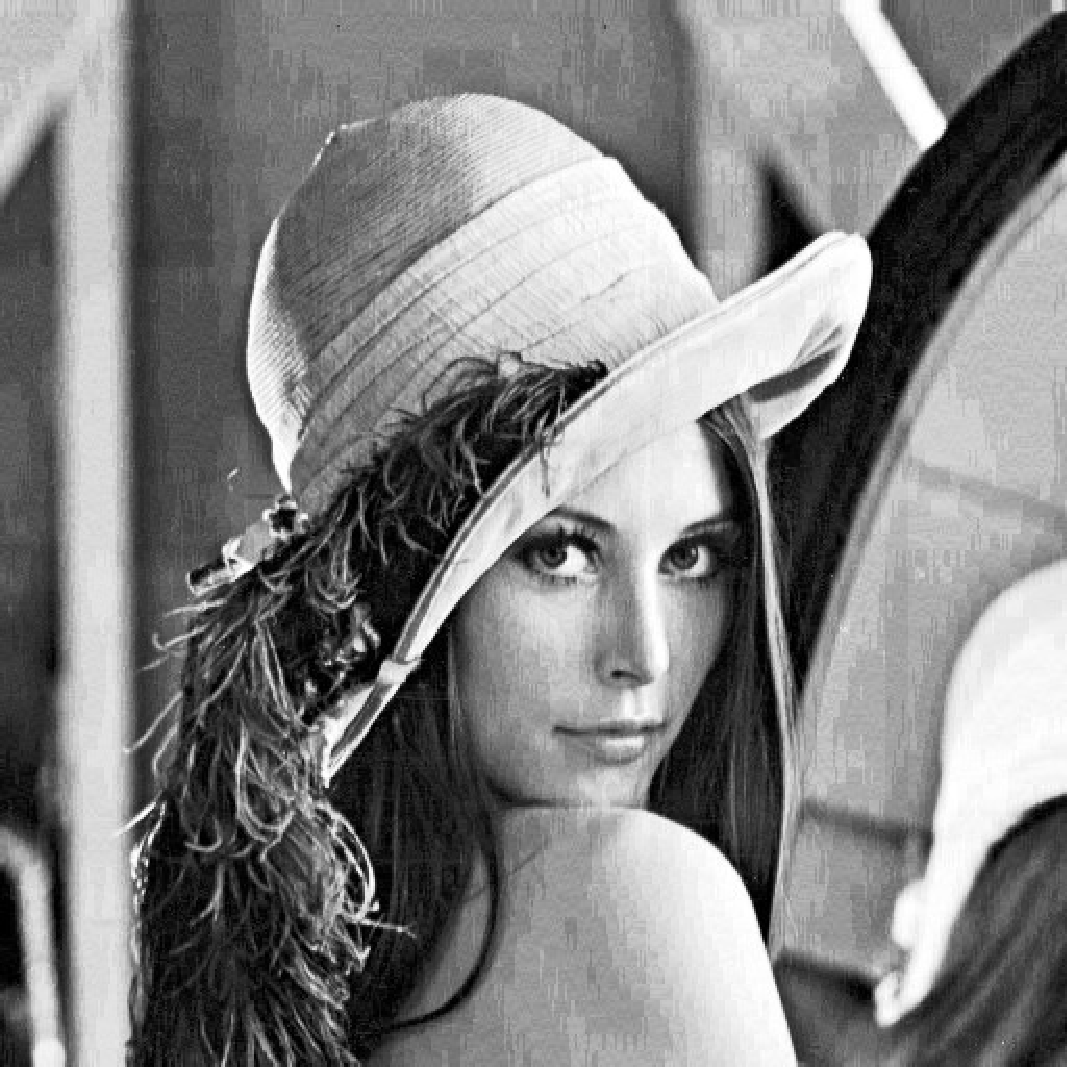
\includegraphics[scale=0.1]{obrazky/equalize}
\end{minipage} &
\begin{minipage}[c]{.15\textwidth}
\ 
  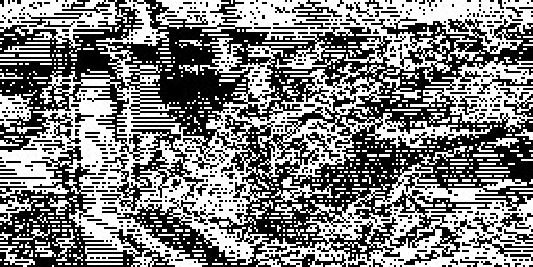
\includegraphics[scale=0.25]{obrazky/equalize-wm}
\end{minipage} \\ \hline
\end{tabular}
\caption{Útoky vylepšením obrazu}
\end{table}

\clearpage
\section{Transformácie obrazu} \label{transform}
Tranformácie obrazu sú častým prípadom spracovávania obrazu. V~tejto časti overíme odolnosť vodoznaku proti zmene veľkosti obrázku a rotácii.
\begin{table}[h]
\centering
\label{transform-table}
\begin{tabular}{llcc}
\hline
\multicolumn{1}{c}{\textbf{Typ útoku}} & \multicolumn{1}{c}{\textbf{NC}} & \multicolumn{1}{c}{\textbf{Vodoznačený obraz}} & \multicolumn{1}{c}{\textbf{Extrahovaný vodoznak}} \\ \hline
Zmenšenie o~25\%                       & 0.298 & 
\begin{minipage}[c]{.1\textwidth}
\ 
  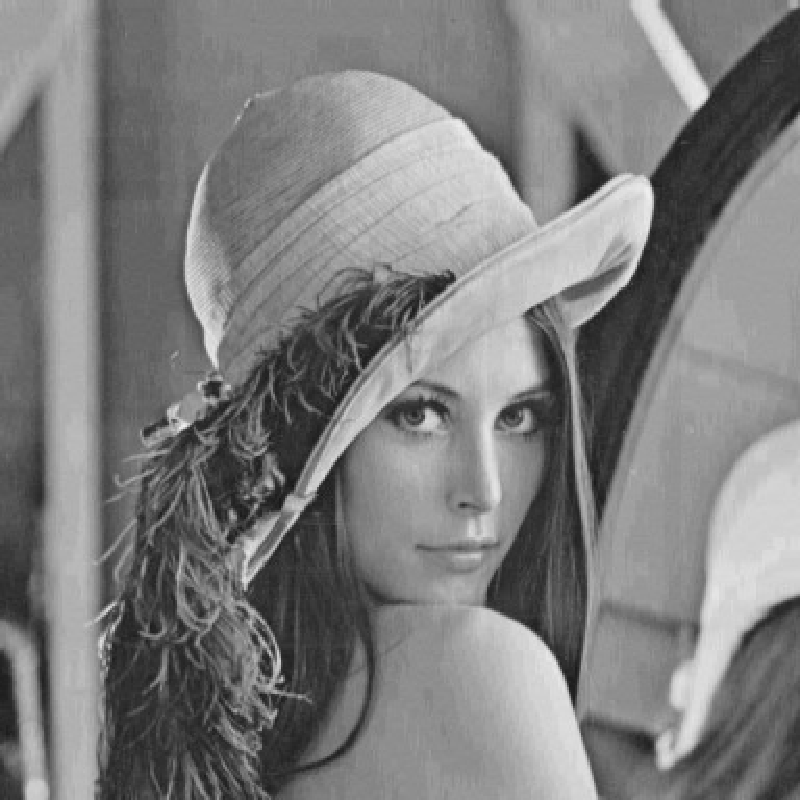
\includegraphics[scale=0.1]{obrazky/scale75}
\end{minipage}
 &
 \begin{minipage}[c]{.15\textwidth}
   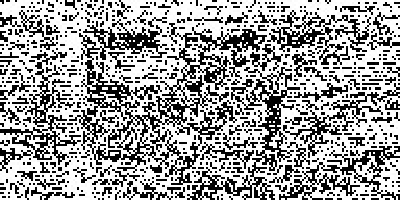
\includegraphics[scale=0.25]{obrazky/scale75-wm}
 \end{minipage} \\
Zväčšenie o~25\%                       & 0.390 &
\begin{minipage}[c]{.1\textwidth}
\ 
  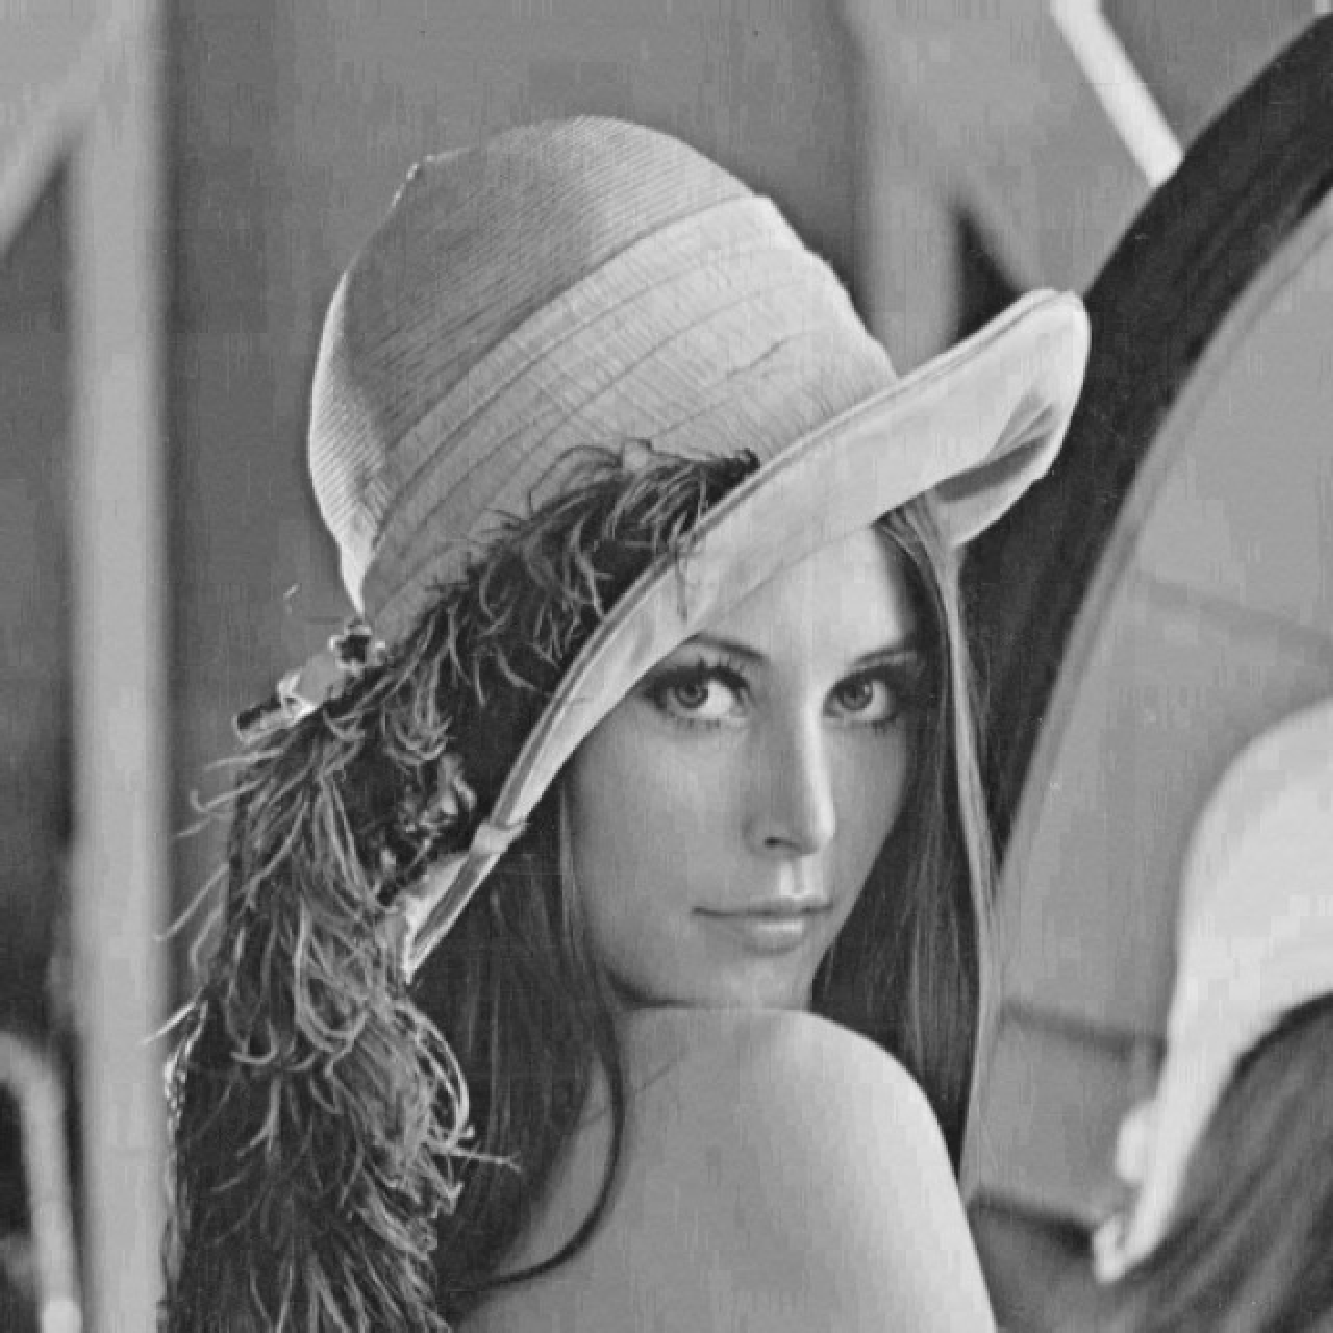
\includegraphics[scale=0.1]{obrazky/scale125}
\end{minipage}
 &
 \begin{minipage}[c]{.15\textwidth}
   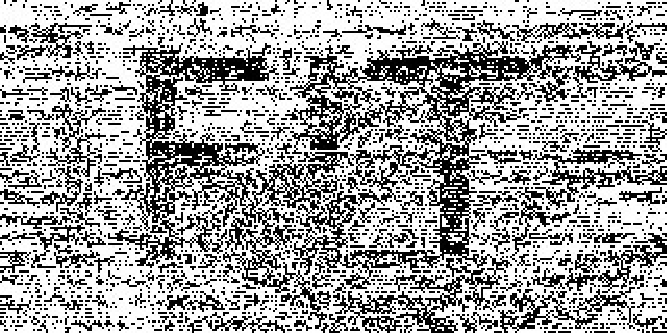
\includegraphics[scale=0.25]{obrazky/scale125-wm}
 \end{minipage} \\
Rotácia o~5 stupňov                    & 0.014 &
\begin{minipage}[c]{.1\textwidth}
\ 
  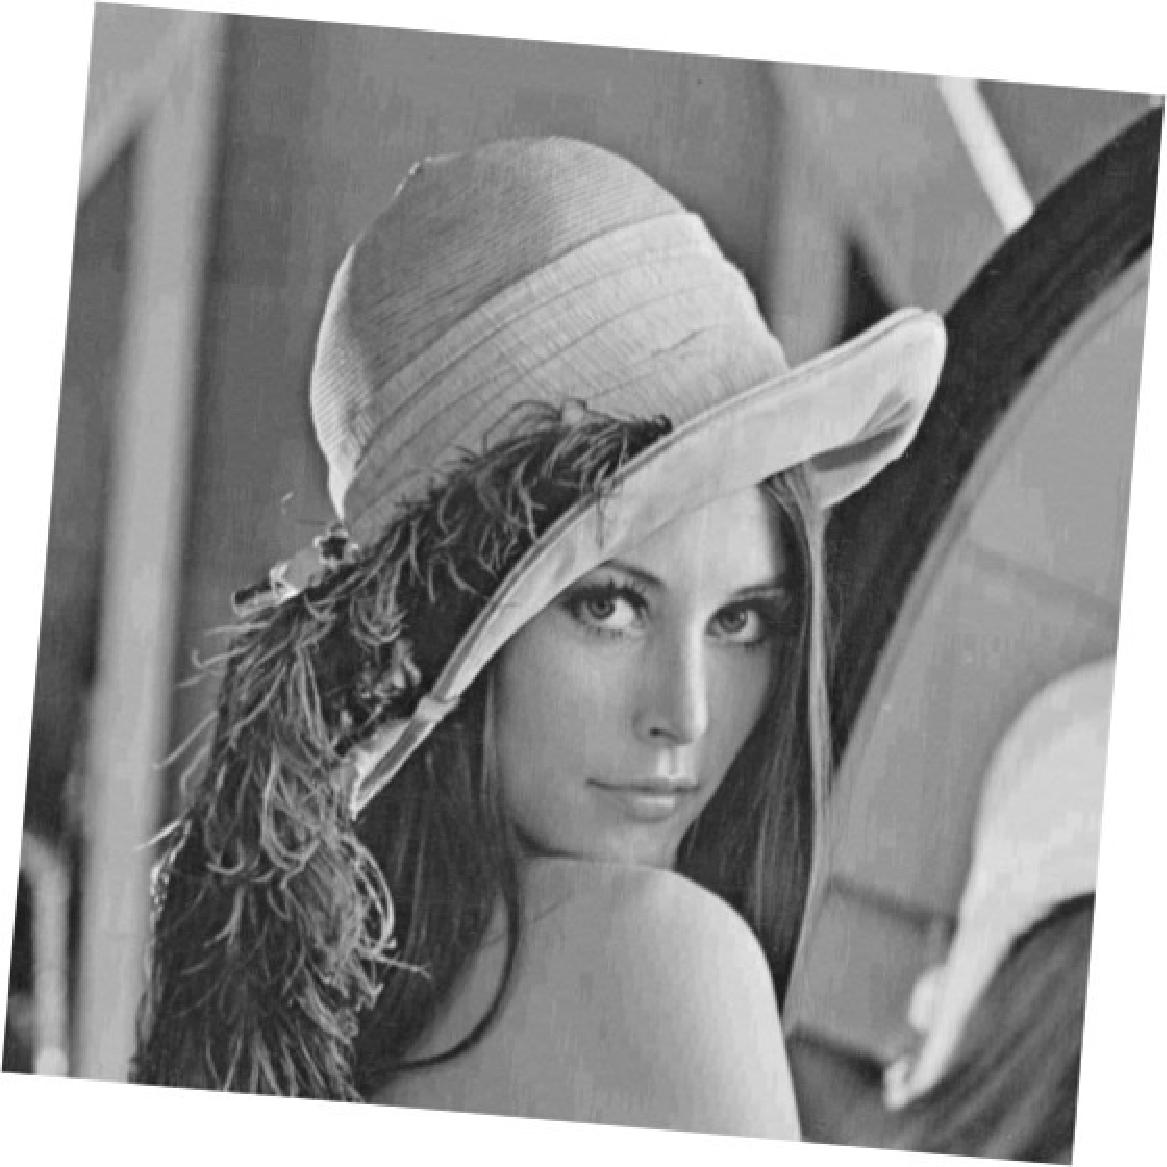
\includegraphics[scale=0.1]{obrazky/rotation5}
\end{minipage}
 &
 \begin{minipage}[c]{.15\textwidth}
   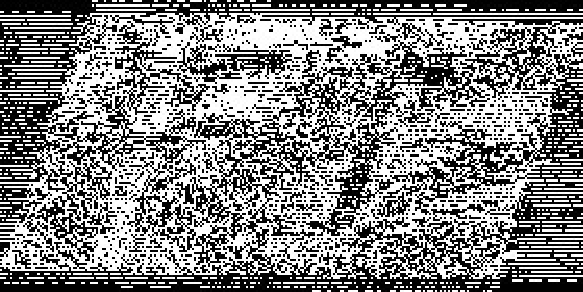
\includegraphics[scale=0.25]{obrazky/rotation5-wm}
 \end{minipage} \\
Rotácia o~10 stupňov                   & 0.160 &
\begin{minipage}[c]{.1\textwidth}
\ 
  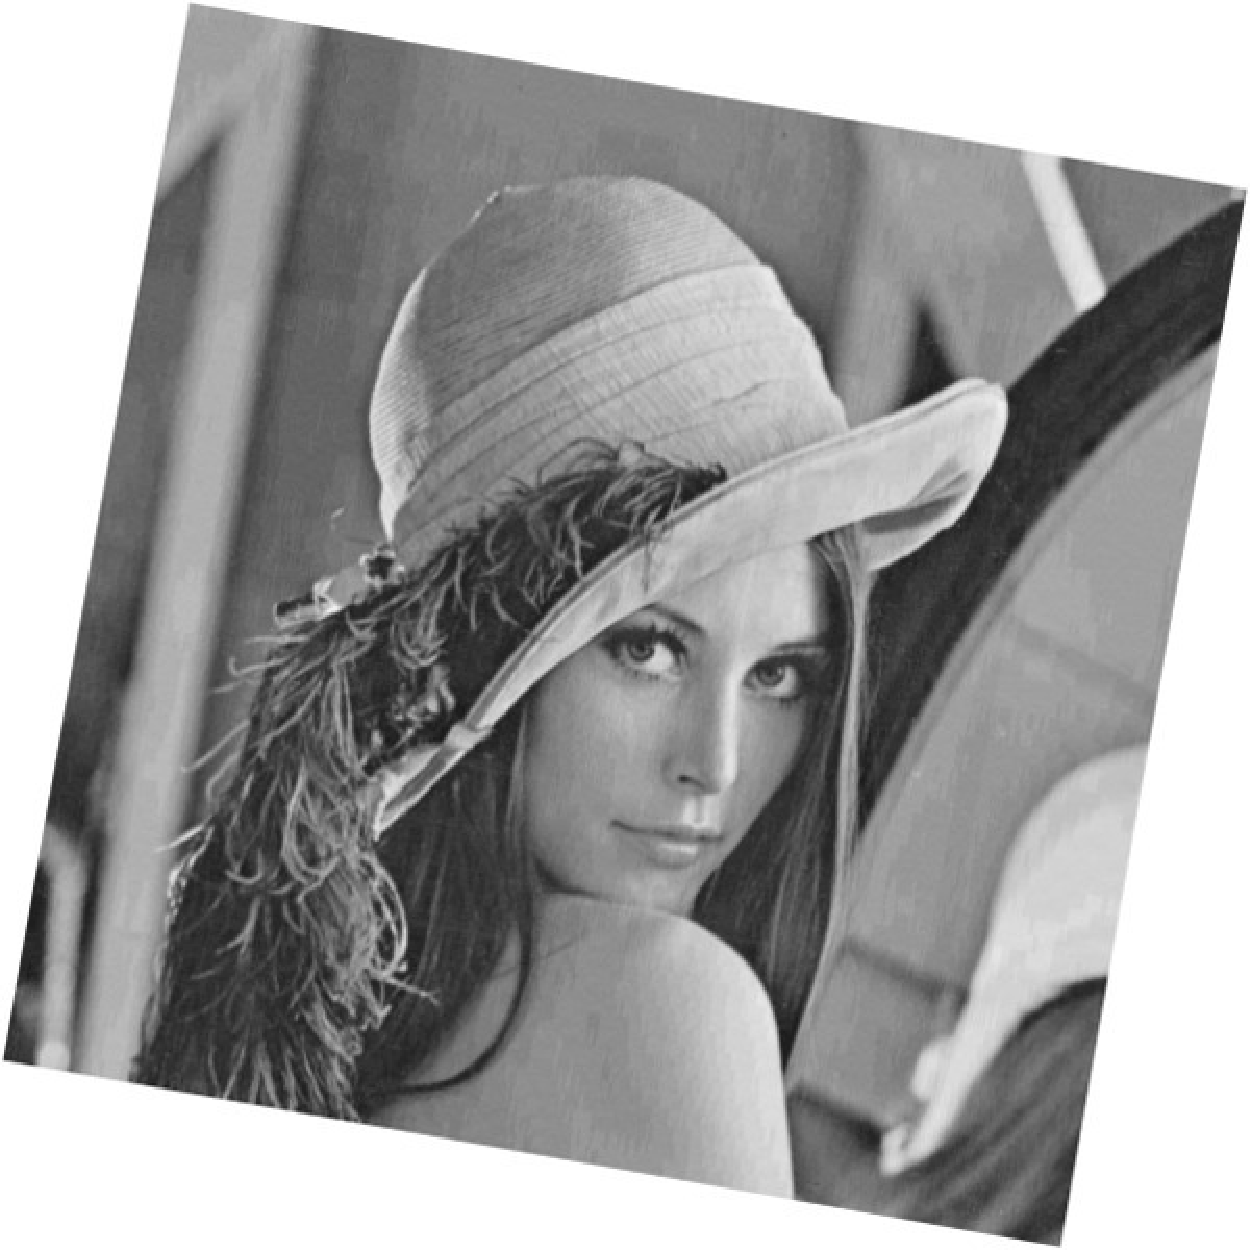
\includegraphics[scale=0.1]{obrazky/rotation10}
\end{minipage}
 &
 \begin{minipage}[c]{.15\textwidth}
   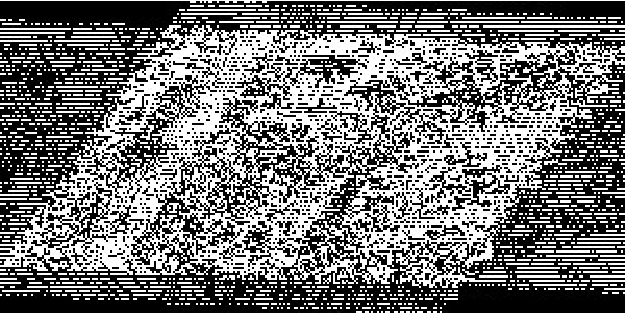
\includegraphics[scale=0.25]{obrazky/rotation10-wm}
 \end{minipage} \\ \hline
\end{tabular}
\caption{Útoky transformáciou obrazu}
\end{table}

Pri týchto útokoch bolo určenie normalizovanej korelácie zložitejšie ako pri iných útokoch. Dôvodom je, že zmenou veľkosti nosného obrázku sa zmenia aj rozmery extrahovaného vodoznaku. Pre vyriešenie tohto problému sme po extrahovaní vodoznaku tento vodoznaka zväčšili alebo zmenšili na základe pomeru v~akom sa zmenil nosný obraz. Po zmene veľkosti vodoznaku sme však narazili na ďalší problém, zmenou veľkosti vodoznak nadobudol aj iné hodnoty ako 0 alebo 255. Riešením je následné prahovanie extrahovaného vodoznaku.

Ako vidíme v~tabuľke, pri každom z~týchto útokov bol vodoznak značne poškodený. Najúspešnejšie dopadol test na zväčšenie vodoznačeného obrazu o~25\% s~$NC=0,390$. Naopak najhoršie dopadli obidva útoky rotáciou obrazu. Pri rotáciách je výsledný vodoznak neidentifikovateľný.

\clearpage
\section{Útoky kompresiou} \label{compress}
Stratová JPEG kompresia dokáže poškodiť vložený vodoznak natoľko, že ho nebude možné rozoznať. Práve preto sme sa pri testovaní zamerali aj na tento typ útoku. Nasledujúca tabuľka \ref{compress-table} zobrazuje výsledky pri rôznej úrovni kompresie.
\begin{table}[h]
\centering
\label{compress-table}
\begin{tabular}{llcc}
\hline
\multicolumn{1}{c}{\textbf{Typ útoku}} & \multicolumn{1}{c}{\textbf{NC}} & \multicolumn{1}{c}{\textbf{Vodoznačený obraz}} & \multicolumn{1}{c}{\textbf{Extrahovaný vodoznak}} \\ \hline
JPEG 70\%                       & 0.614 &
\begin{minipage}[c]{.1\textwidth}
\ 
  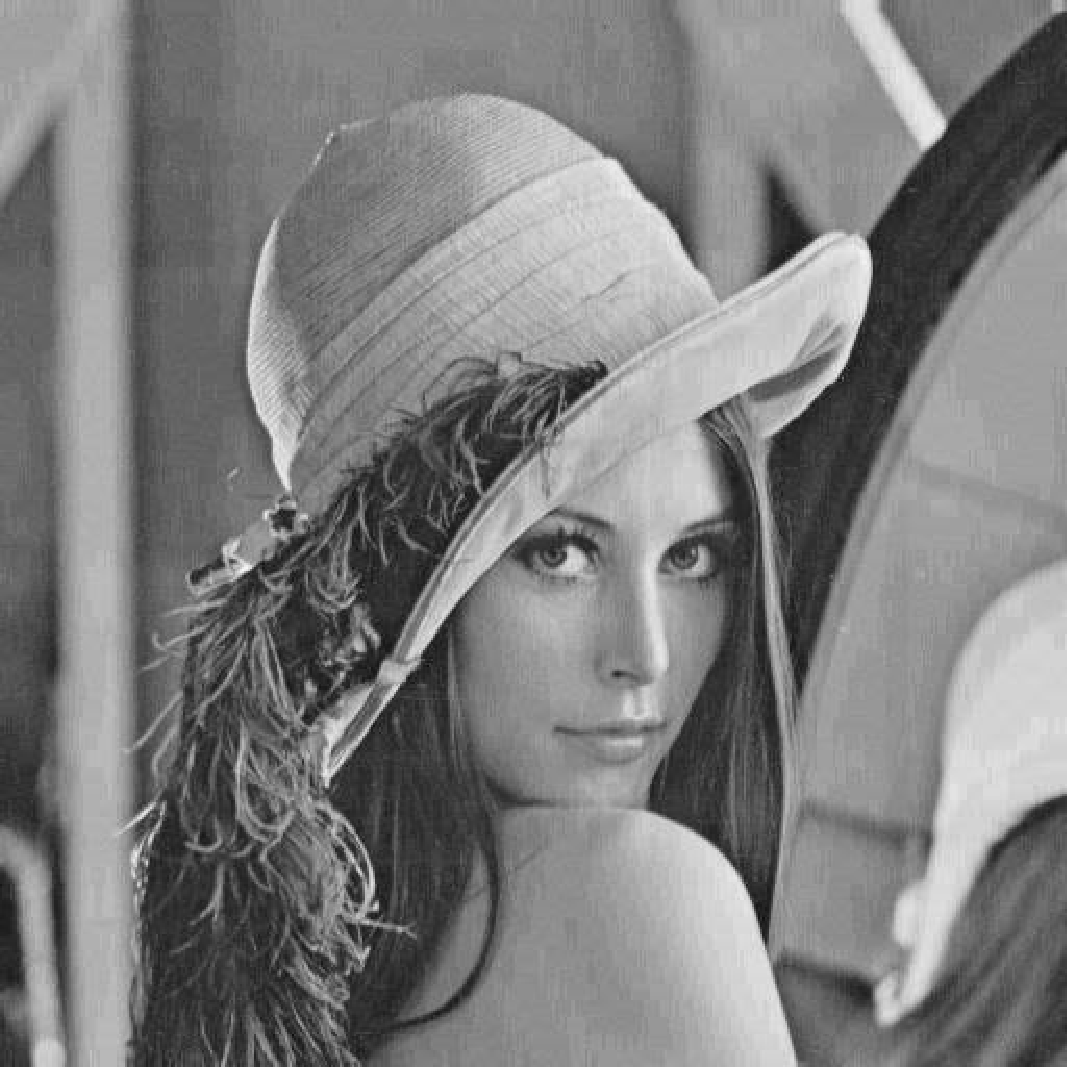
\includegraphics[scale=0.1]{obrazky/jpeg70}
\end{minipage} &
 \begin{minipage}[c]{.15\textwidth}
   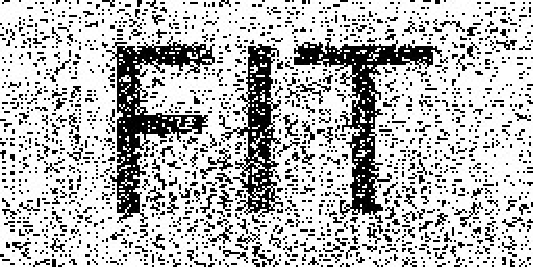
\includegraphics[scale=0.25]{obrazky/jpeg70-wm}
 \end{minipage}  \\
JPEG 50\%                       & 0.429 &
\begin{minipage}[c]{.1\textwidth}
\ 
  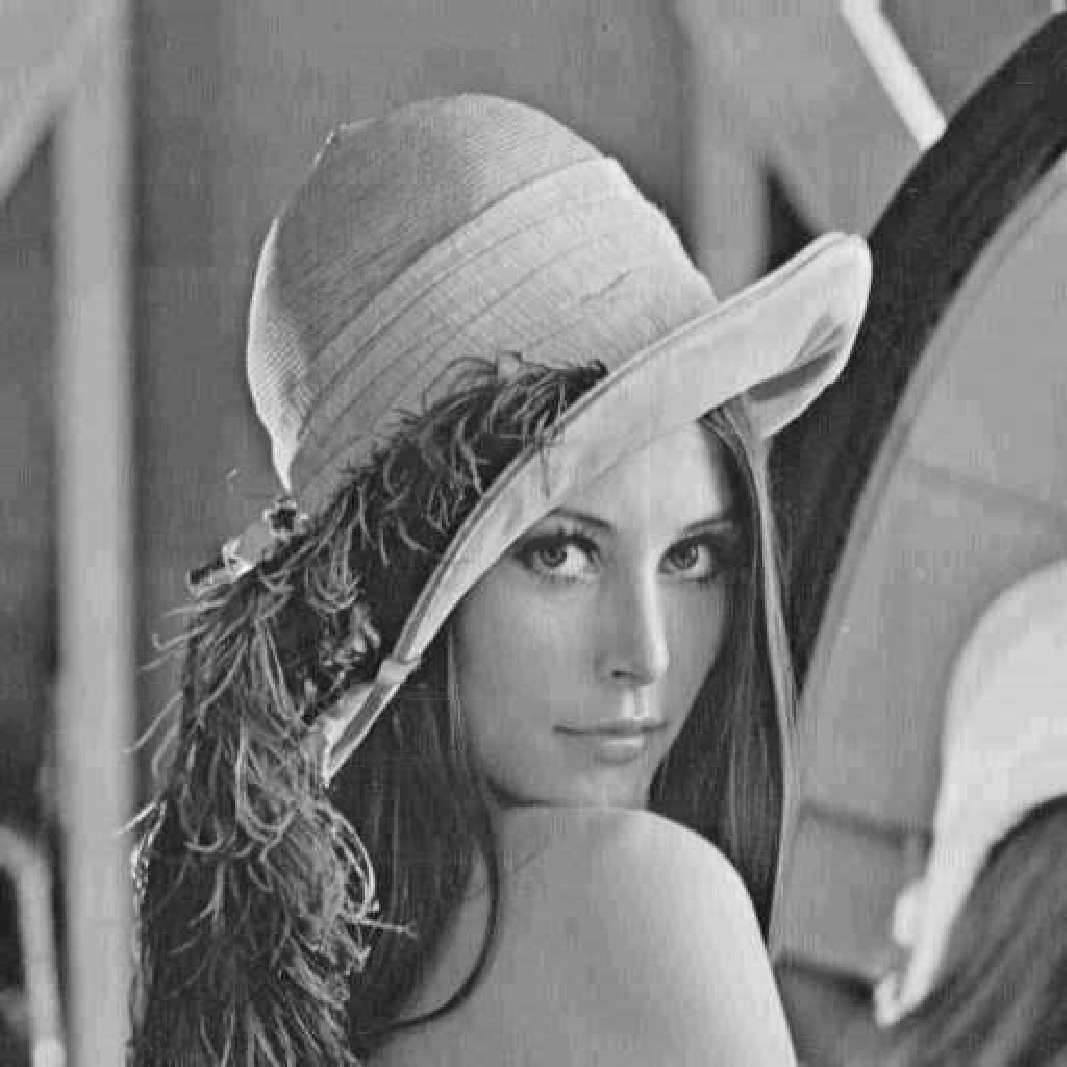
\includegraphics[scale=0.1]{obrazky/jpeg50}
\end{minipage} &
 \begin{minipage}[c]{.15\textwidth}
   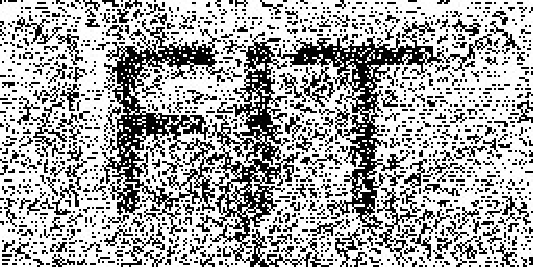
\includegraphics[scale=0.25]{obrazky/jpeg50-wm}
 \end{minipage}  \\
JPEG 30\%                     & 0.298 &
\begin{minipage}[c]{.1\textwidth}
\ 
  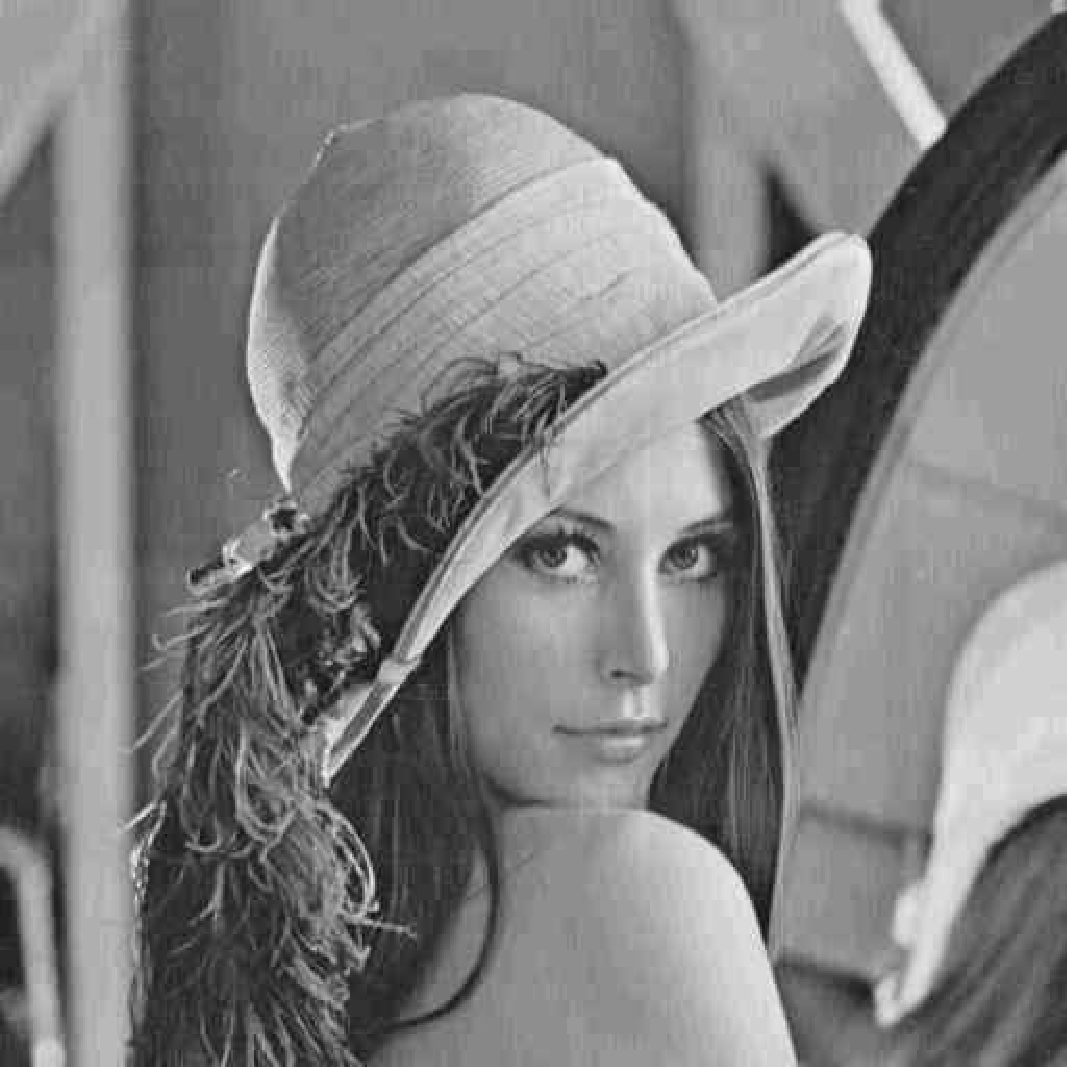
\includegraphics[scale=0.1]{obrazky/jpeg30}
\end{minipage} &
 \begin{minipage}[c]{.15\textwidth}
   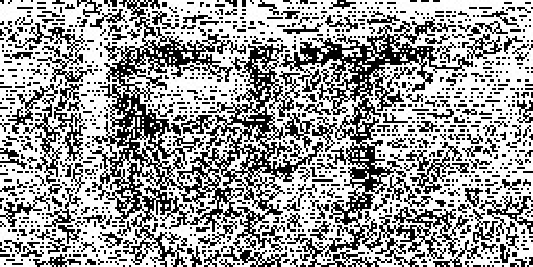
\includegraphics[scale=0.25]{obrazky/jpeg30-wm}
 \end{minipage}  \\
JPEG 20\%                    & 0.193 &
\begin{minipage}[c]{.1\textwidth}
\ 
  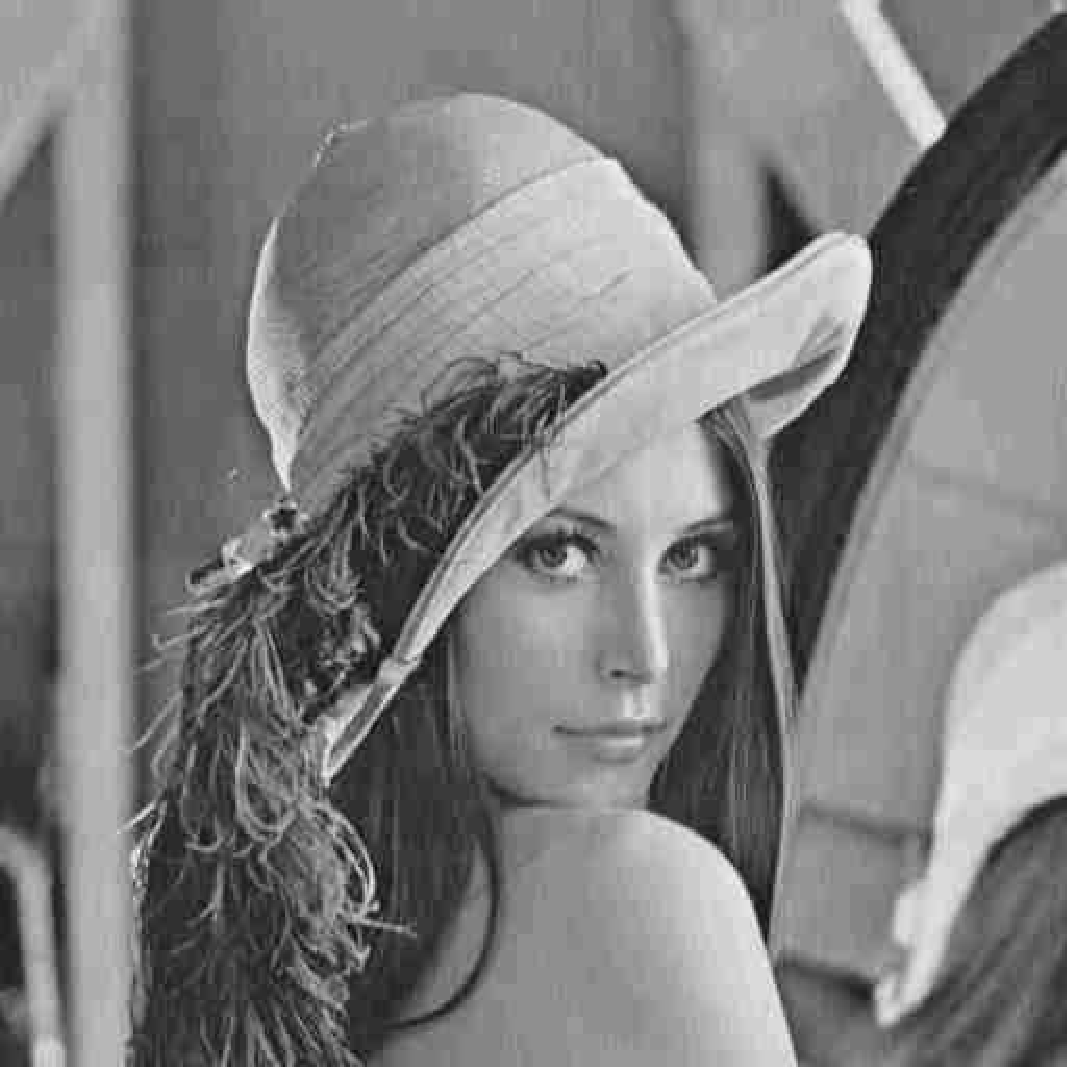
\includegraphics[scale=0.1]{obrazky/jpeg20}
\end{minipage} &
 \begin{minipage}[c]{.15\textwidth}
   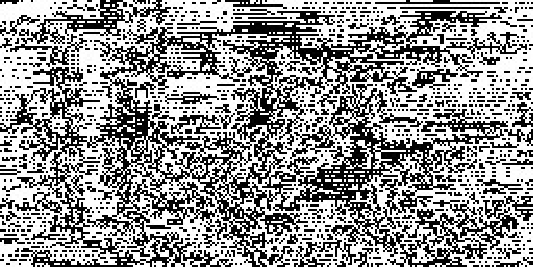
\includegraphics[scale=0.25]{obrazky/jpeg20-wm}
 \end{minipage}  \\ \hline
\end{tabular}
\caption{Útoky JPEG kompresiou}
\end{table}

Po útokoch stratovou JPEG kompresiou môžeme skonštatovať, že ešte pri 50\% kompresii sme schopní rozpoznať extrahovaný vodoznak. Pri zvolení silnejšej kompresie je vodoznak už vážnejšie poškodený.

\chapter{Záver}